\documentclass[a4paper,titlepage]{scrartcl}
\pagestyle{plain}
\usepackage[utf8]{inputenc}
\usepackage[T1]{fontenc}
\usepackage[german]{babel}
\usepackage{units}
\usepackage{floatrow}
\usepackage{amsmath,amssymb,amstext}
\usepackage{pgfplots,pgfplotstable}
\usepackage{numprint}
\usepackage{graphicx}

\newfloatcommand{capbtabbox}{table}[][\FBwidth]
\numberwithin{equation}{section}

\title{Versuch P2-59: Operationsverstärker\\Auswertung}
\author{Gruppe Di-22\\Genti Saliu, Jonas Müller}
\date{02. Juni 2014}

\begin{document}

\begin{titlepage}
\maketitle
\thispagestyle{empty}
\end{titlepage}

\newpage
\pagenumbering{roman}
\tableofcontents

\newpage
\pagenumbering{arabic}

\section{Emitterschaltung}
\subsection{Einstufiger gleichstromgekoppelter Transistorverstärker}
Gemäß der Schaltskizze aus unserer Vorbereitung wurde im Versuch die Emitterschaltung gebaut. Statt $\unit[5]{\mu F}$-Kondensatoren (sie waren im Labor nicht vorhanden) setzten wir $\unit[4.7]{\mu F}$-Kondensatoren in unserer Schaltung ein.
\subsection{Bestimmung der Verstärkung mit Dreieckspannung}
Es sollte in diesem Versuch die Verstärkung der im vergangenen Versuch gebauten Schaltung bestimmt werden. Dazu haben wir während der Versuchsdurchführung dem Verstärker eine Dreieckspannung ($f=\unit[1]{kHz}$) mit verschiedenen Amplituden ($3 V_{SS}- 10 V_{SS}$) zugeführt und uns die Ausgangsamplituden notiert (s. Tabelle \ref{tab:aufgabe12}).
\begin{table}[H]
\begin{tabular}{c|c|c}
	$U_E$ $(mV)$ & $U_A$ $(V)$ & Verstärkung $\beta$ \\
	\hline
	26 & -3.76 & -144.61 \\
	34.8 & -5.2 & -149.42 \\
	60 & -9.12 & -152 \\
\end{tabular}
\caption{Verstärkung der Emitterschaltung}
\label{tab:aufgabe12}
\end{table}
Das Ausgangssignal ist gegenüber dem Eingangssignal um $\unit[90]{^\circ}$ phasenverschoben, d.h. die Verstärkung ist negativ. Die mittlere Verstärkung beträgt $\beta=-148.68$.
\begin{figure}[H]
	\centering
	\begin{tabular}{@{}r@{}}
		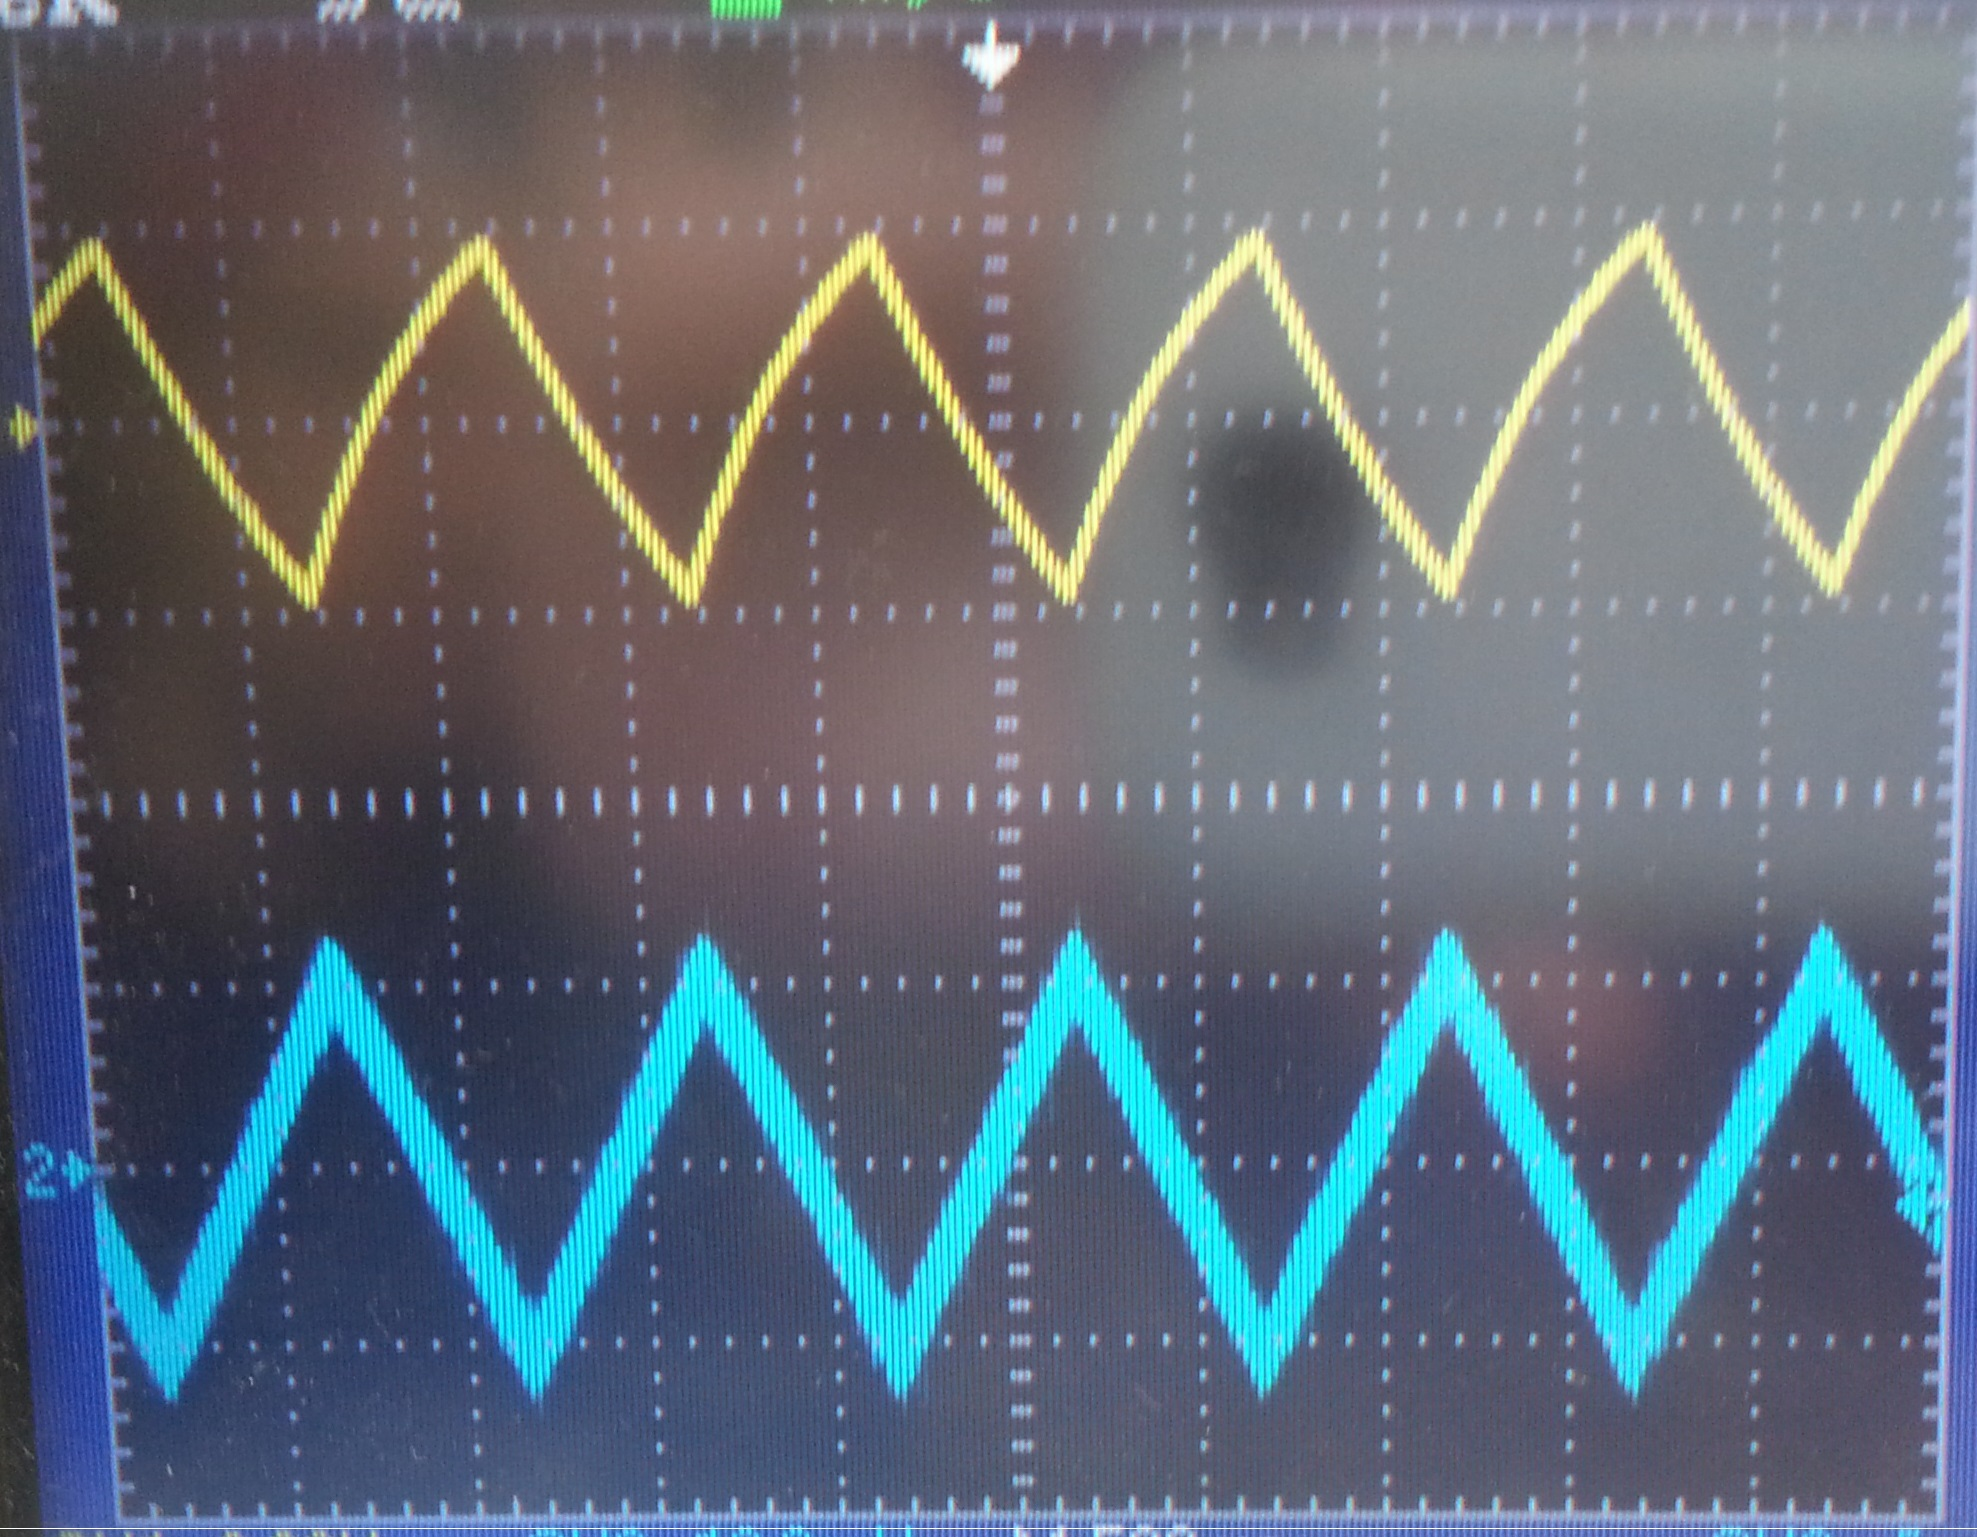
\includegraphics[width=0.5\textwidth]{bilder/aufgabe12.jpg}\\
	\end{tabular}
	\caption{Eingangs- und Ausgangssignal}
	\label{fig:aufgabe12}
\end{figure}
\subsection{Bestimmung der Verstärkung des stromgegenkoppeltes Verstärkers ohne Emitterkondensator}
Wir haben nun den Emitterkondensator $C_e$ entfernt und die gleichen Messungen wie in Aufgabe 1.2 wiederholt (s. Tabelle \ref{tab:aufgabe13}).
\begin{table}[H]
\begin{tabular}{c|c|c}
	$U_E$ $(mV)$ & $U_A$ $(mV)$ & Verstärkung $\beta$ \\
	\hline
	156 & -700 & -4.49 \\
	235 & -1050 & -4.47 \\
	404 & -1840 & -4.55 \\
\end{tabular}
\caption{Verstärkung der Emitterschaltung ohne $C_e$}
\label{tab:aufgabe13}
\end{table}
Der Mittelwert der Verstärkung beträgt damit -4.5, was fast der theoretischen, in der Vorbereitung bestimmten (-4.7) entspricht.
\subsection{Bestimmung der Verstärkung des strom- und gleichstromgegekoppelten Verstärkers für verschiedene Frequenzen}
Es wurden in diesem Versuch die Eingangs- und Ausgangssignale für verschiedene Frequenzen, jeweils für den strom- und gleichstromgegengekoppelten Verstärker gemessen, um daraus die Verstärkung und deren Verlauf in Abhängigkeit von der Frequenz zu bestimmen. Diese sind jeweils in Abbildung \ref{fig:aufgabe14a} und \ref{fig:aufgabe14b} aufgeführt.
\begin{figure}[H]
	\centering
	\begin{tabular}{@{}r@{}}
		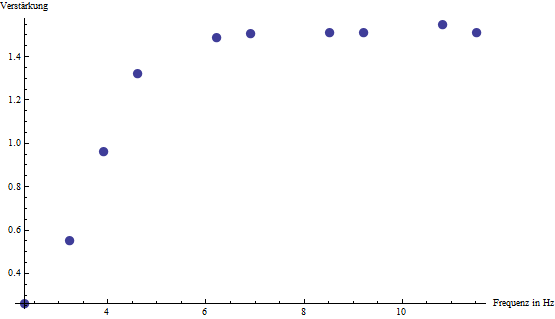
\includegraphics[width=0.9\textwidth]{bilder/aufgabe14-stromgegengekoppelt.png}\\
	\end{tabular}
	\caption{Abhängigkeit der Verstärkung von der Frequenz für die stromgegengekoppelte Schaltung}
	\label{fig:aufgabe14a}
\end{figure}
\begin{figure}[H]
	\centering
	\begin{tabular}{@{}r@{}}
		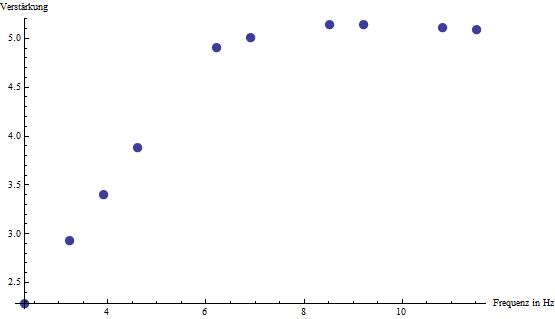
\includegraphics[width=0.9\textwidth]{bilder/aufgabe14-gleichstromgegengekoppelt.png}\\
	\end{tabular}
	\caption{Abhängigkeit der Verstärkung von der Frequenz für die gleichstromgegengekoppelte Schaltung}
	\label{fig:aufgabe14b}
\end{figure}
Es fällt auf, dass beide Verstärkungsformen mit höheren Frequenzen zu einer Sättigungsverstärkung streben.\\ \\
Außerdem ist die Verstärkung bei Stromkopplung deutlich geringer als bei Gleichstromkopplung, da beim Letzteren der Kondensator als Hochpass wirkt (hochfrequente Signale können den Widerstand umgehen).\\ \\
Zusätzlich sieht man in Abbildung \ref{fig:aufgabe14a} nochmal die experimentelle Bestätigung des theoretischen Verstärkungsfaktors für den stromgegengekoppelten Verstärker.
\section{Grundschaltung eines Operationsverstärkers}
\subsection{Nichtinvertierender Verstärker}
Es sollte in diesem Versuch ein nichtinvertierender Verstärker mit \emph{etwa zehnfacher Verstärkung} gebaut werden und überprüft werden, ob tatsächlich die Verstärkung der Erwartung entspricht. Mit den im Versuch verwendeten Widerständen sollte die Verstärkung laut Vorbereitung $\beta = 11$ betragen:
\begin{equation*}
v=1+\frac{R_1}{R_2}=1+\frac{\unit[10]{k \Omega}}{\unit[1]{k \Omega}}=11
\end{equation*}
Wir haben folgende Werte gemessen:
\begin{table}[H]
\begin{tabular}{c|c|c}
	$U_E$ (mV) & $U_A$ (V) & Verstärkung $\beta$ \\
	\hline
	368 & 4.08 & 11.09 \\
\end{tabular}
\caption{Überprüfung des nichtinvertierenden Verstärkers}
\label{tab:aufgabe13}
\end{table}
\begin{figure}[H]
	\centering
	\begin{tabular}{@{}r@{}}
		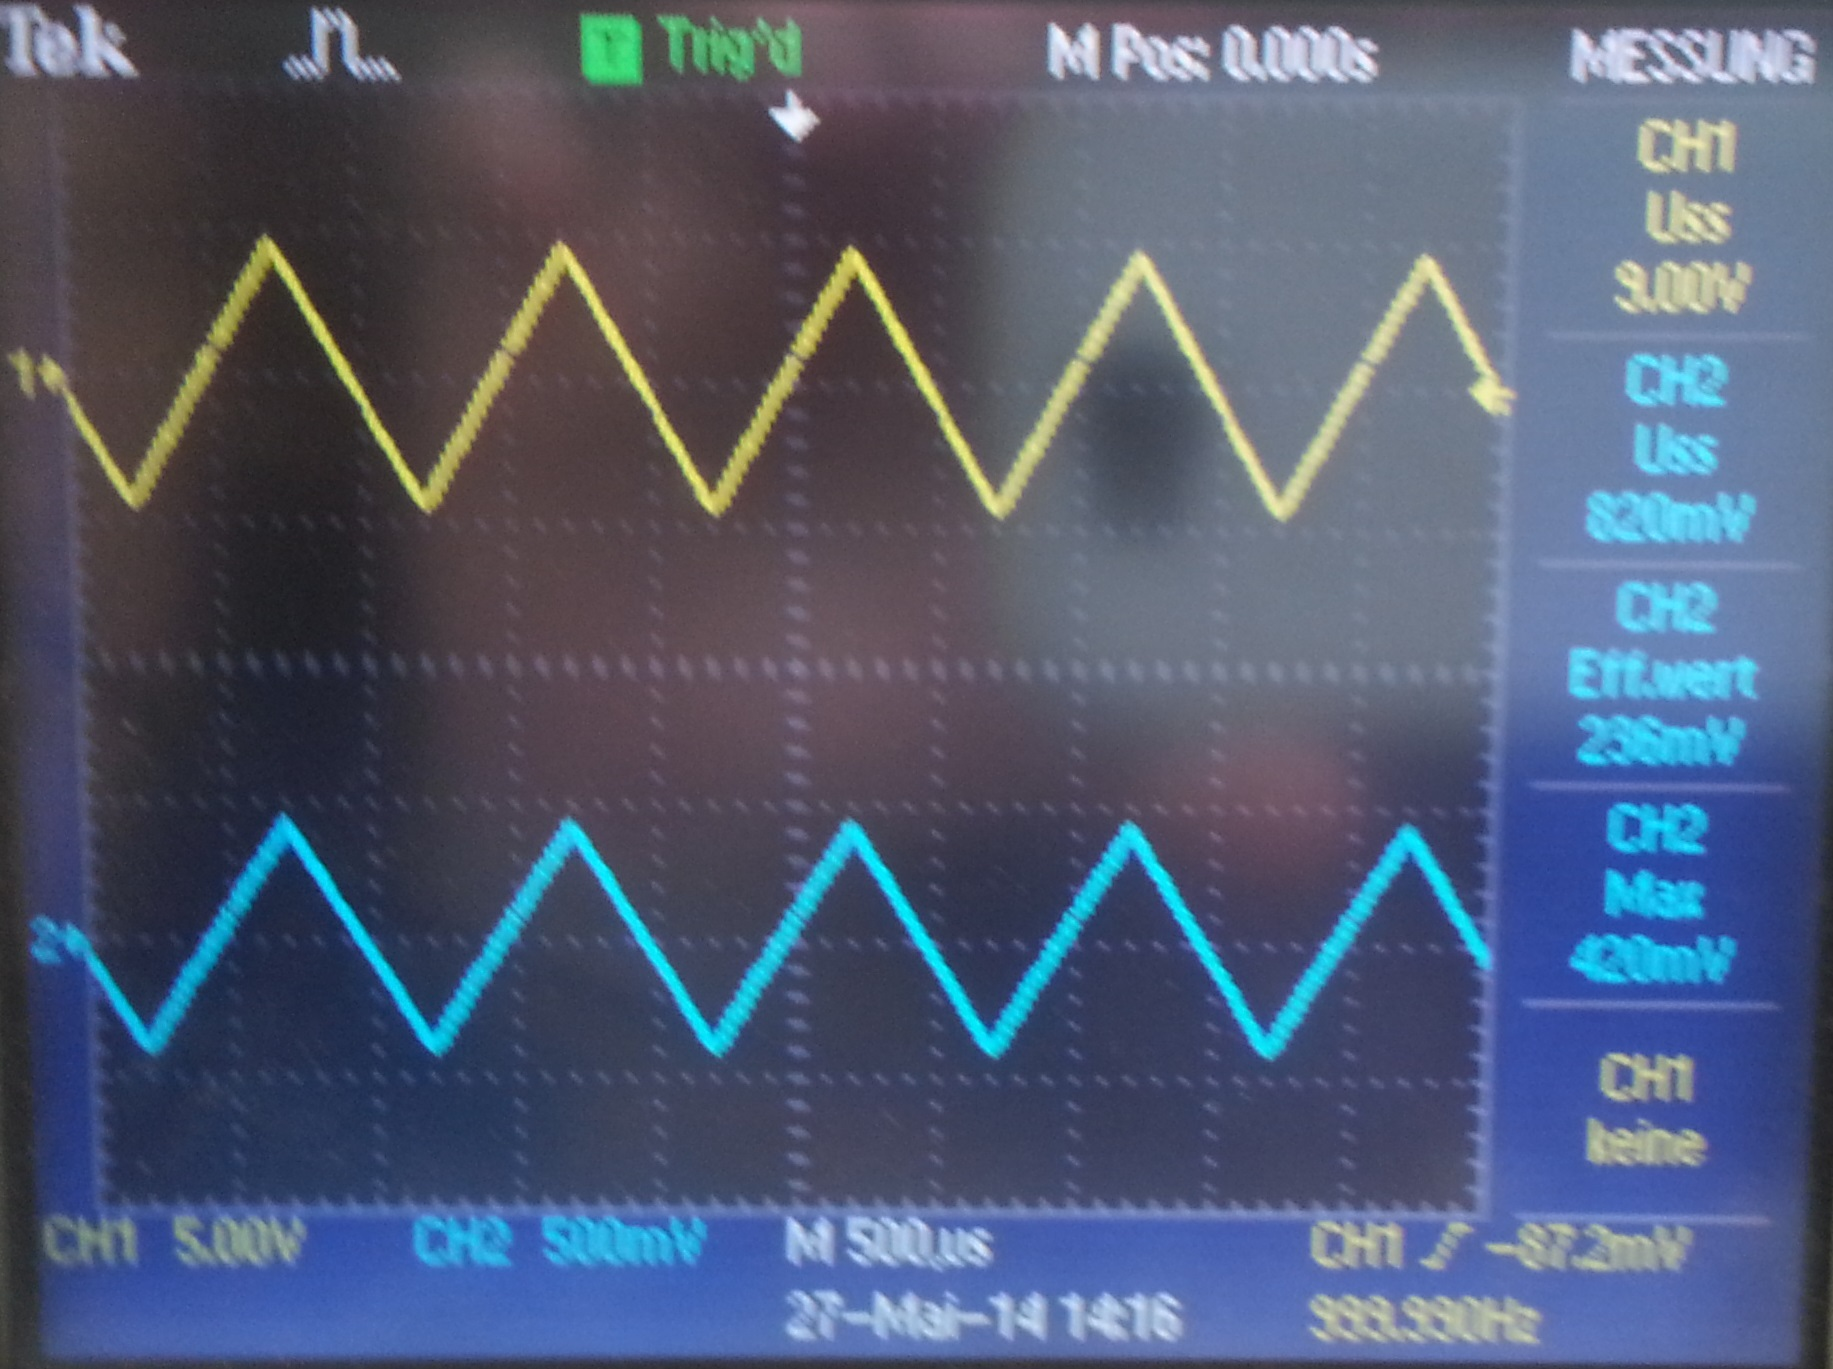
\includegraphics[width=0.58\textwidth]{bilder/aufgabe21.jpg}\\
	\end{tabular}
	\caption{Kennlinie des nichtinvertierenden Verstärkers}
	\label{fig:aufgabe14b}
\end{figure}
\subsection{Demonstration des hohen Eingangs- und kleinen Ausgangswiderstands}
Ein idealer Operationsverstärker zeichnet sich durch unendlichen Eingangswiderstand und keinen/sehr kleinen Ausgangswiderstand aus (die 3 goldenen Regeln).  Wir sollten in diesem Versuch feststellen, wie nah der gebaute Verstärker am idealen OPV ankommt.
\begin{description}
\item[Eingangswiderstand $R_E$] Gemäß Vorbereitung, wurde ein Messwiderstand $R_M=\unit[1]{M \Omega}$ in Reihe zum Eingang $U_E$ angeschlossen und wir maßen den Spannungsabfall $U_M$. Daraus können wir nun den Eingangswiderstand bestimmen:
\begin{equation*}
R_E=R_M \cdot \left(\frac{U_E}{U_M}-1\right)=\unit[10^6]{\Omega} \cdot \left(\frac{\unit[1.72]{V}}{\unit[33 \cdot 10^{-3}]{V}}-1\right)=\unit[10^6]{\Omega} \cdot (52.12 - 1) = \unit[51.12 \cdot 10^6]{\Omega}
\end{equation*}
Wie erwartet, ist der Eingangswiderstand sehr groß.
\item[Ausgangswiderstand] Wir schlossen dazu ein Potentiometer parallel zum Ausgang und reduzierten dessen Widerstand kontinuierlich, bis die Ausgangsspannung auf die halbe Amplitude sank. An diesem Punkt entsprach der eingestellte Widerstand dem Ausgangswiderstand. Der eingestellte Widerstand war somit $R_A=\unit[302]{\Omega}$.
\end{description}
\subsection{Bestimmung der Verstärkung des stromgegenkoppeltes Verstärkers ohne Emitterkondensator}
Ähnlich wie Aufgabe 1.4, ging es in diesem Versuch um die Abhängigkeit der Verstärkung von der Frequenz zu untersuchen. Dazu legten wir eine Sinuswechselspannung mit Amplitude 0.5 $V_{SS}$ mit verschiedenen Frequenzen am Eingang und betrachteten die Amplitude der Ausgangsspannung. Daraus erhielten wir Schaubild \ref{fig:aufgabe23}:
\begin{figure}[H]
	\centering
	\begin{tabular}{@{}r@{}}
		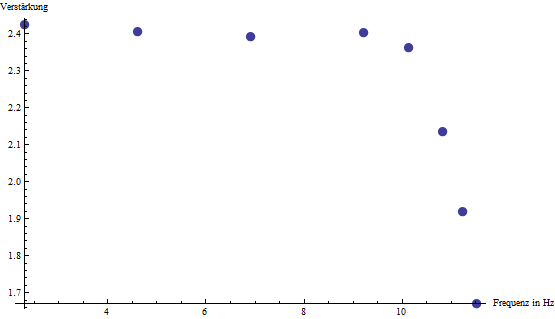
\includegraphics[width=0.7\textwidth]{bilder/aufgabe23.png}\\
	\end{tabular}
	\caption{Verstärkung des nichtinvertierenden Verstärkers}
	\label{fig:aufgabe23}
\end{figure}
Man erkennt, dass mit steigenden Frequenzen, die Verstärkung kleiner wird. Die Gegenkopplung für hohe Frequenzen ist dafür verantwortlich, dass wir
\subsection{Abhängigkeit der Verstärkung von der Frequenz}

\section{Invertierende Grundschaltungen}
\subsection{Invertierter Verstärker}

Wie in der Vorbereitung beschrieben bauten wir einen invertierten Verstärker auf. Mit den verwendeten Bauteilen sollte sich eine zehnfache Verstärkung erkenne lassen. Dies war auch der Fall, wir erhielten:

\begin{equation*}
v= \frac{U_A}{U_E}= \frac{\unit[4.46]{V}}{\unit[0.464]{V}}=10
\end{equation*}

Wobei immer Spitze-Spitze-Werte der Spannung betrachtet wurden. Unser Ergebnis entspricht also sogar genau dem erwarteten Wert.

\begin{figure}[H]
\centering
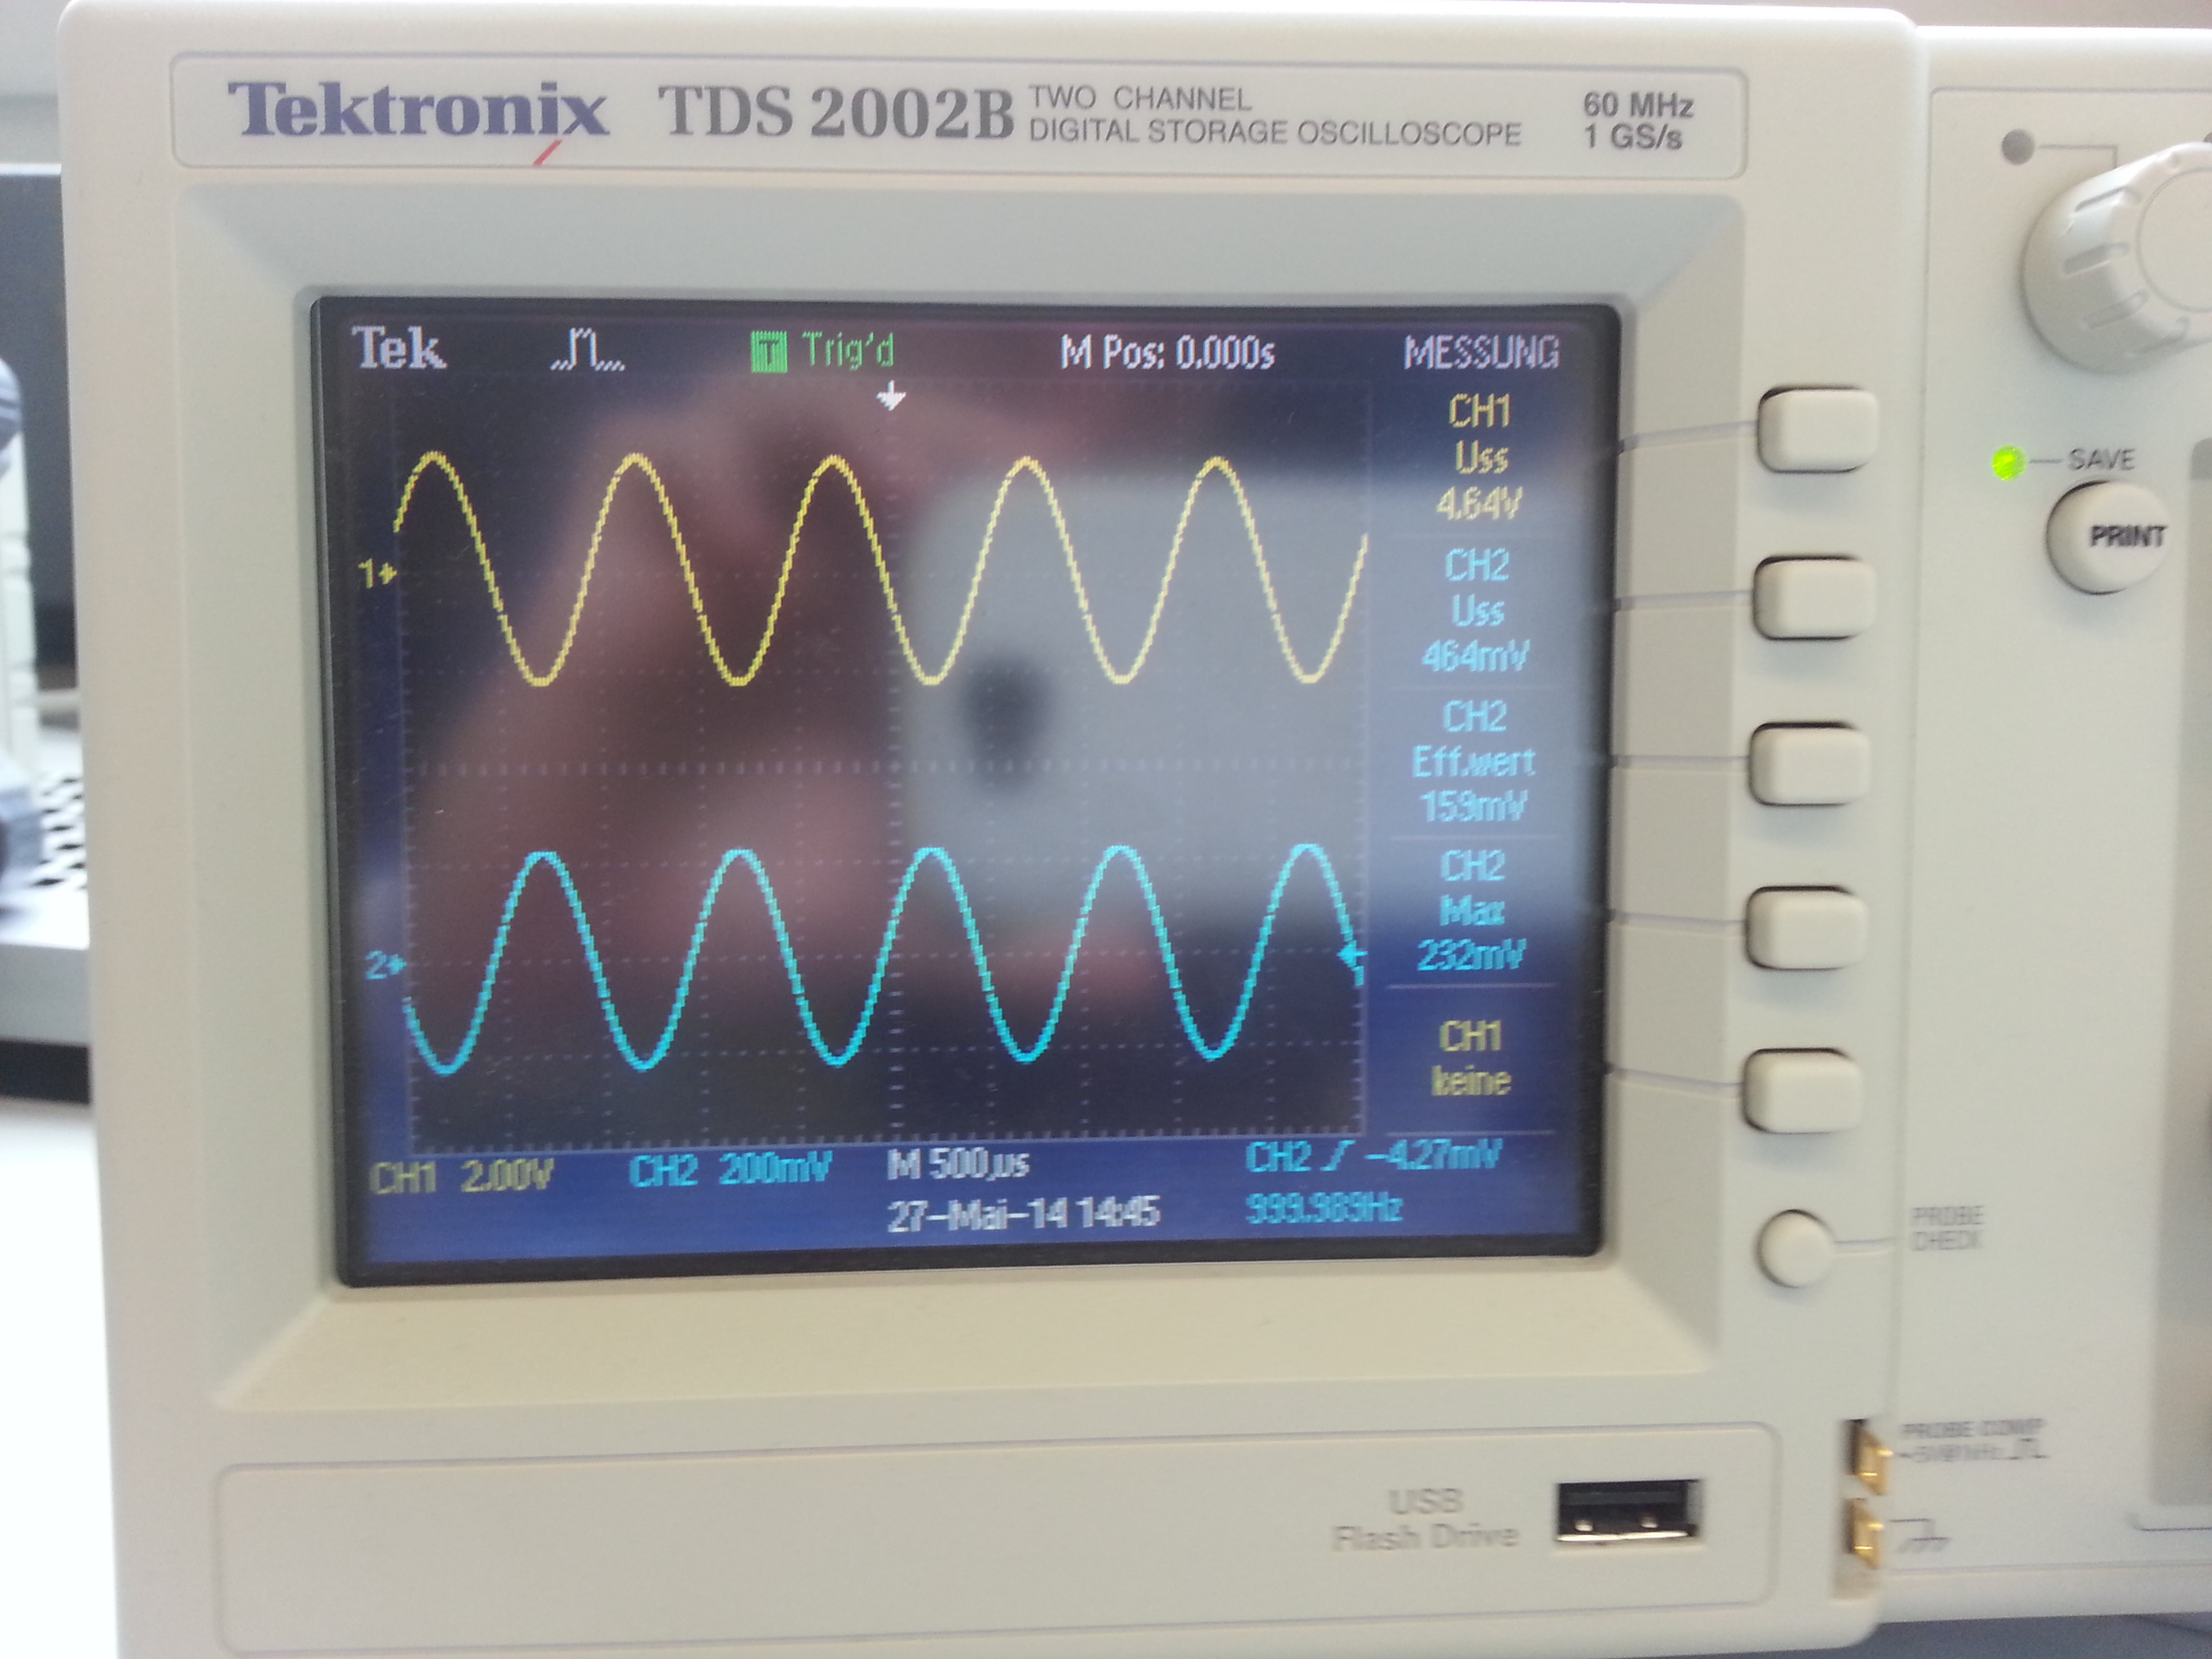
\includegraphics[scale=.08]{bilder/invert_verstaerker.jpg} 
\caption{Oszilloskopbild}
\end{figure}

Man kann auf dem Oszilloskop leicht erkennen, dass Eingangs- und Ausgangssignal unterschiedliche Vorzeichen besitzen.

\subsection{Addierer für zwei Eingangssignale}

Wie in der Vorbereitung beschrieben, wurde ein Addierer für zwei Eingangssignale gebaut. Prinzipiell wären auch mehr Eingänge mit der gleichen Schaltung möglich gewesen. Wir führten den Versuch mit der anderen Praktikumsgruppe durch, da mehrere Funktionsgeneratoren benötigt wurden.\\
Zunächst wählten wir am Eingang eine Rechtecksspannung und eine Sinusspannung bei ungefähr gleicher Frequenz.

\begin{figure}[H]
\centering
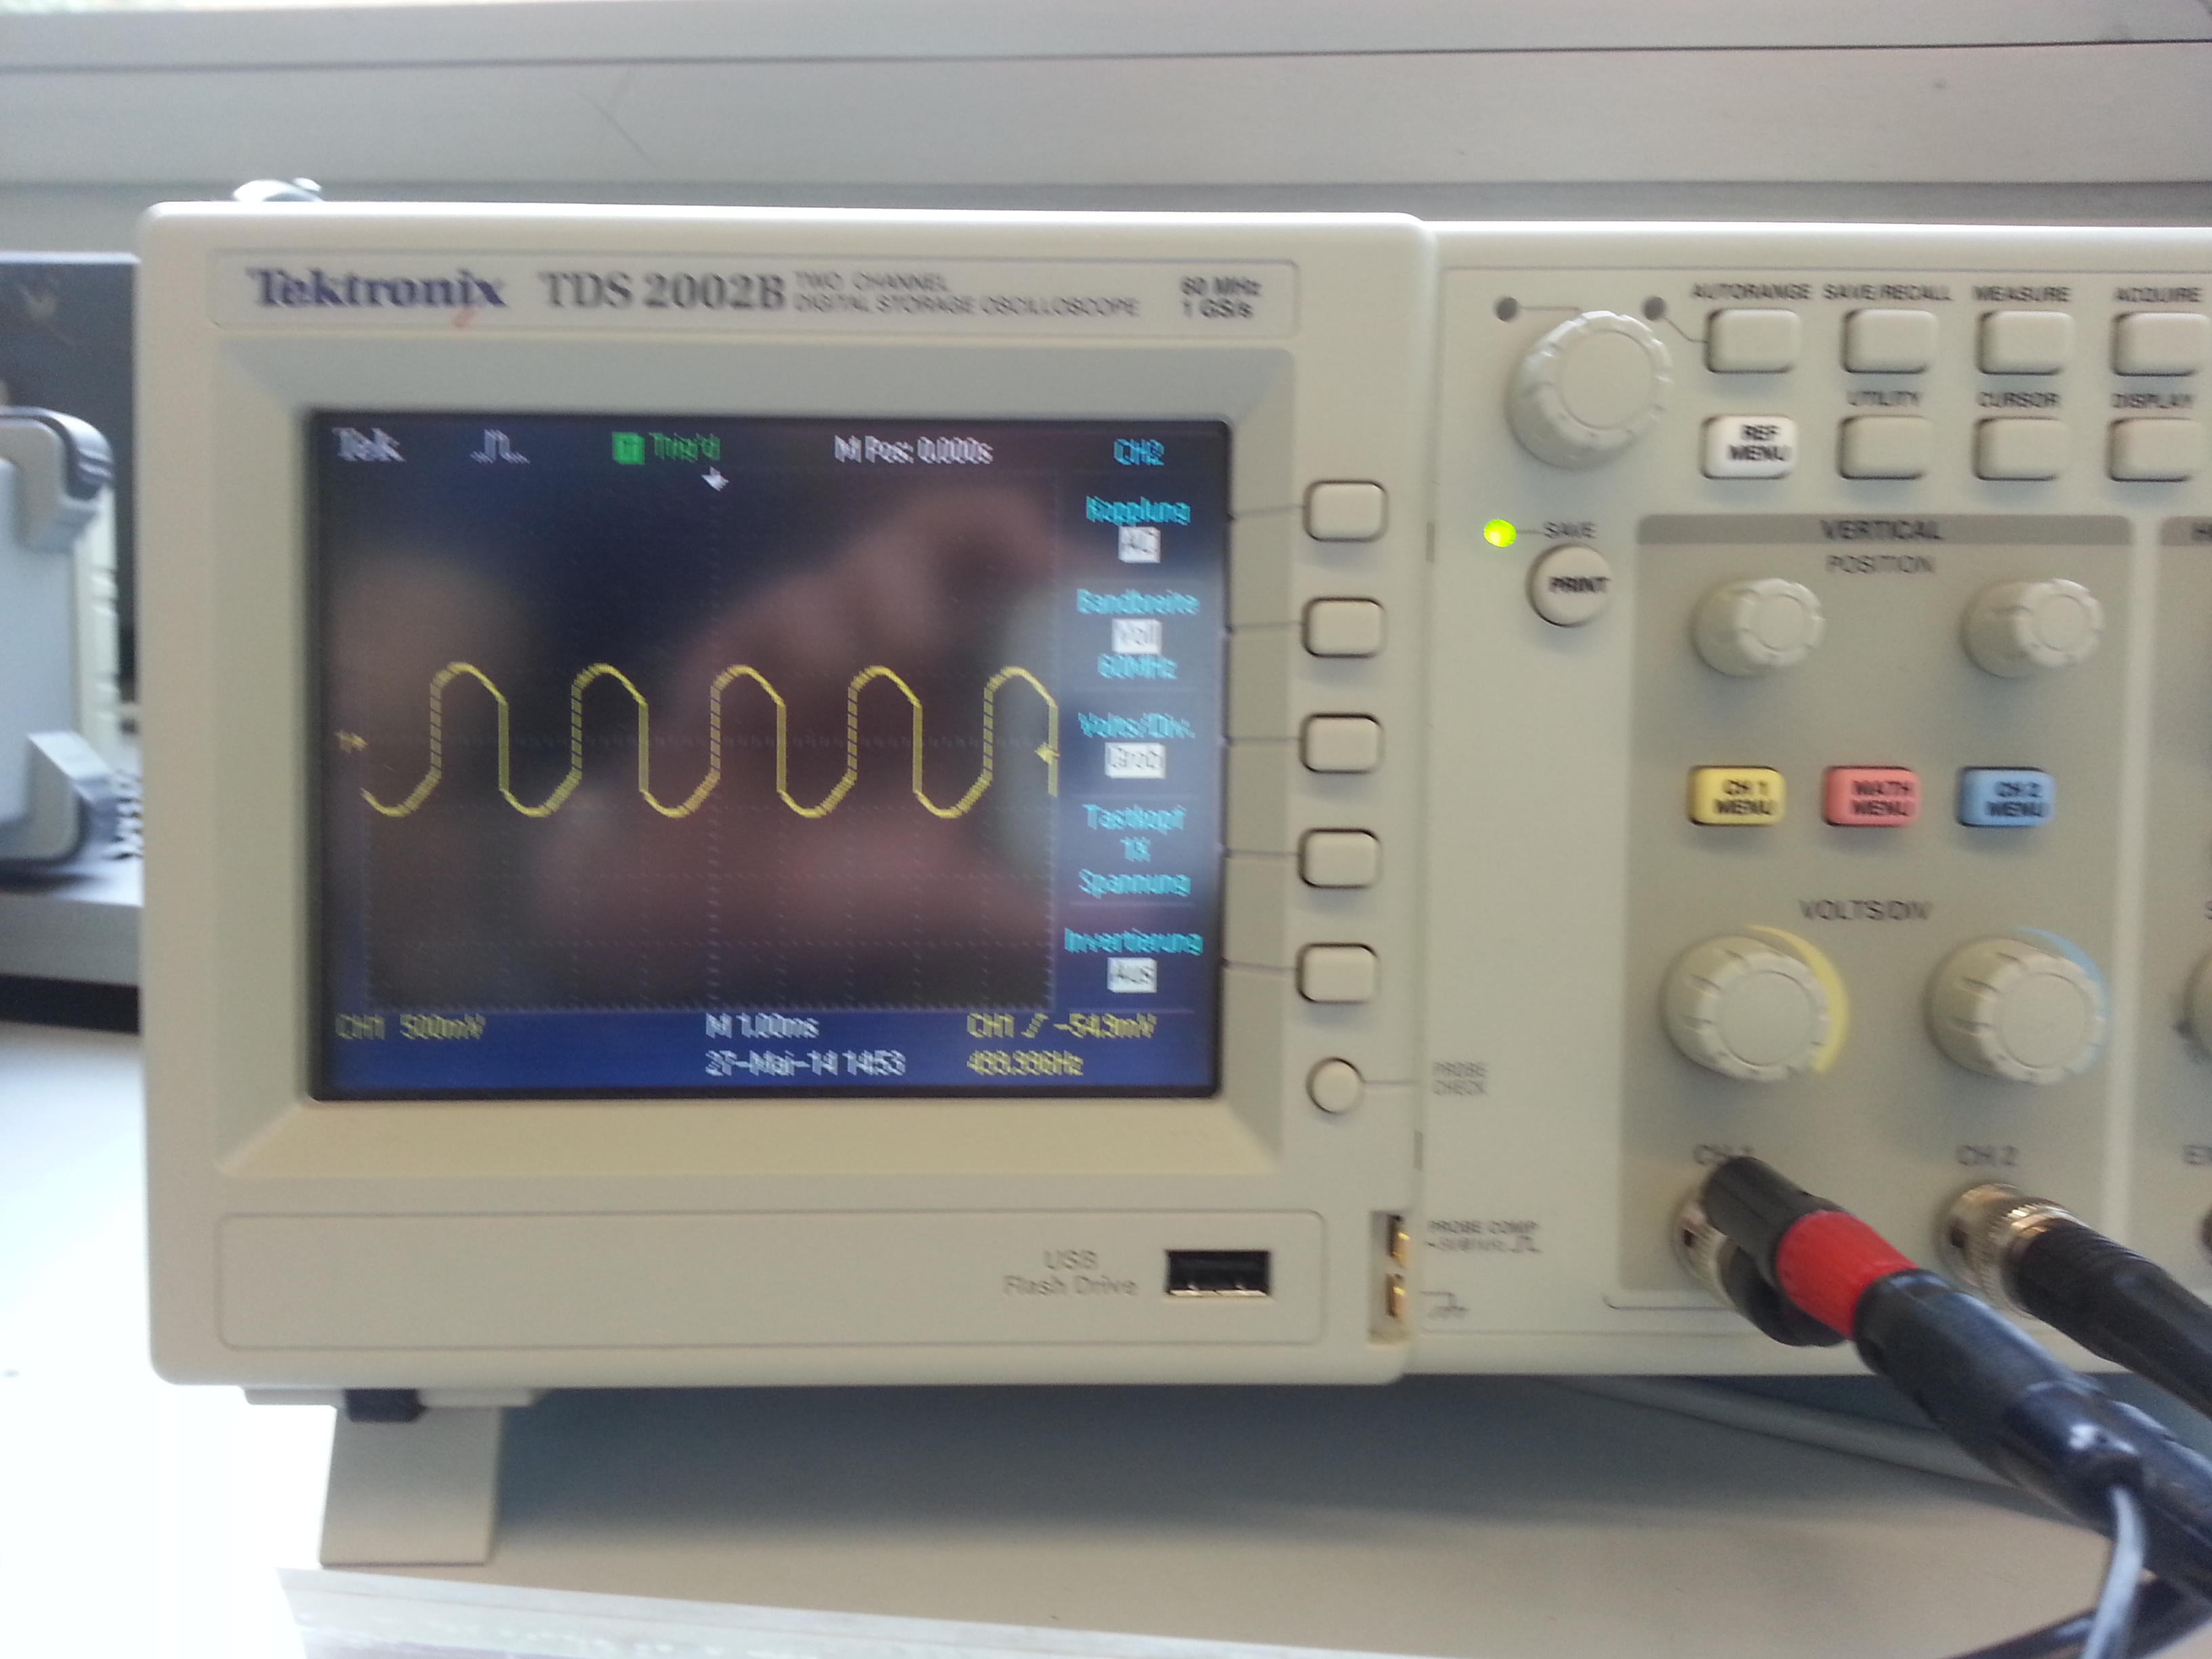
\includegraphics[scale=.08]{bilder/aufgabe_3_2_1.jpg} 
\caption{Oszilloskopbild der Addition von Sinus- und Rechtecksspannung}
\end{figure}

Außerdem addiert wir noch eine Dreiecksspannung mit niedrigerer Frequenz und eine Sinusspannung mit höherer Frequenz. Man kann auf dem Oszilloskopbild gut die Überlagerung der einzelnen Funktionen erkennen.

\begin{figure}[H]
\centering
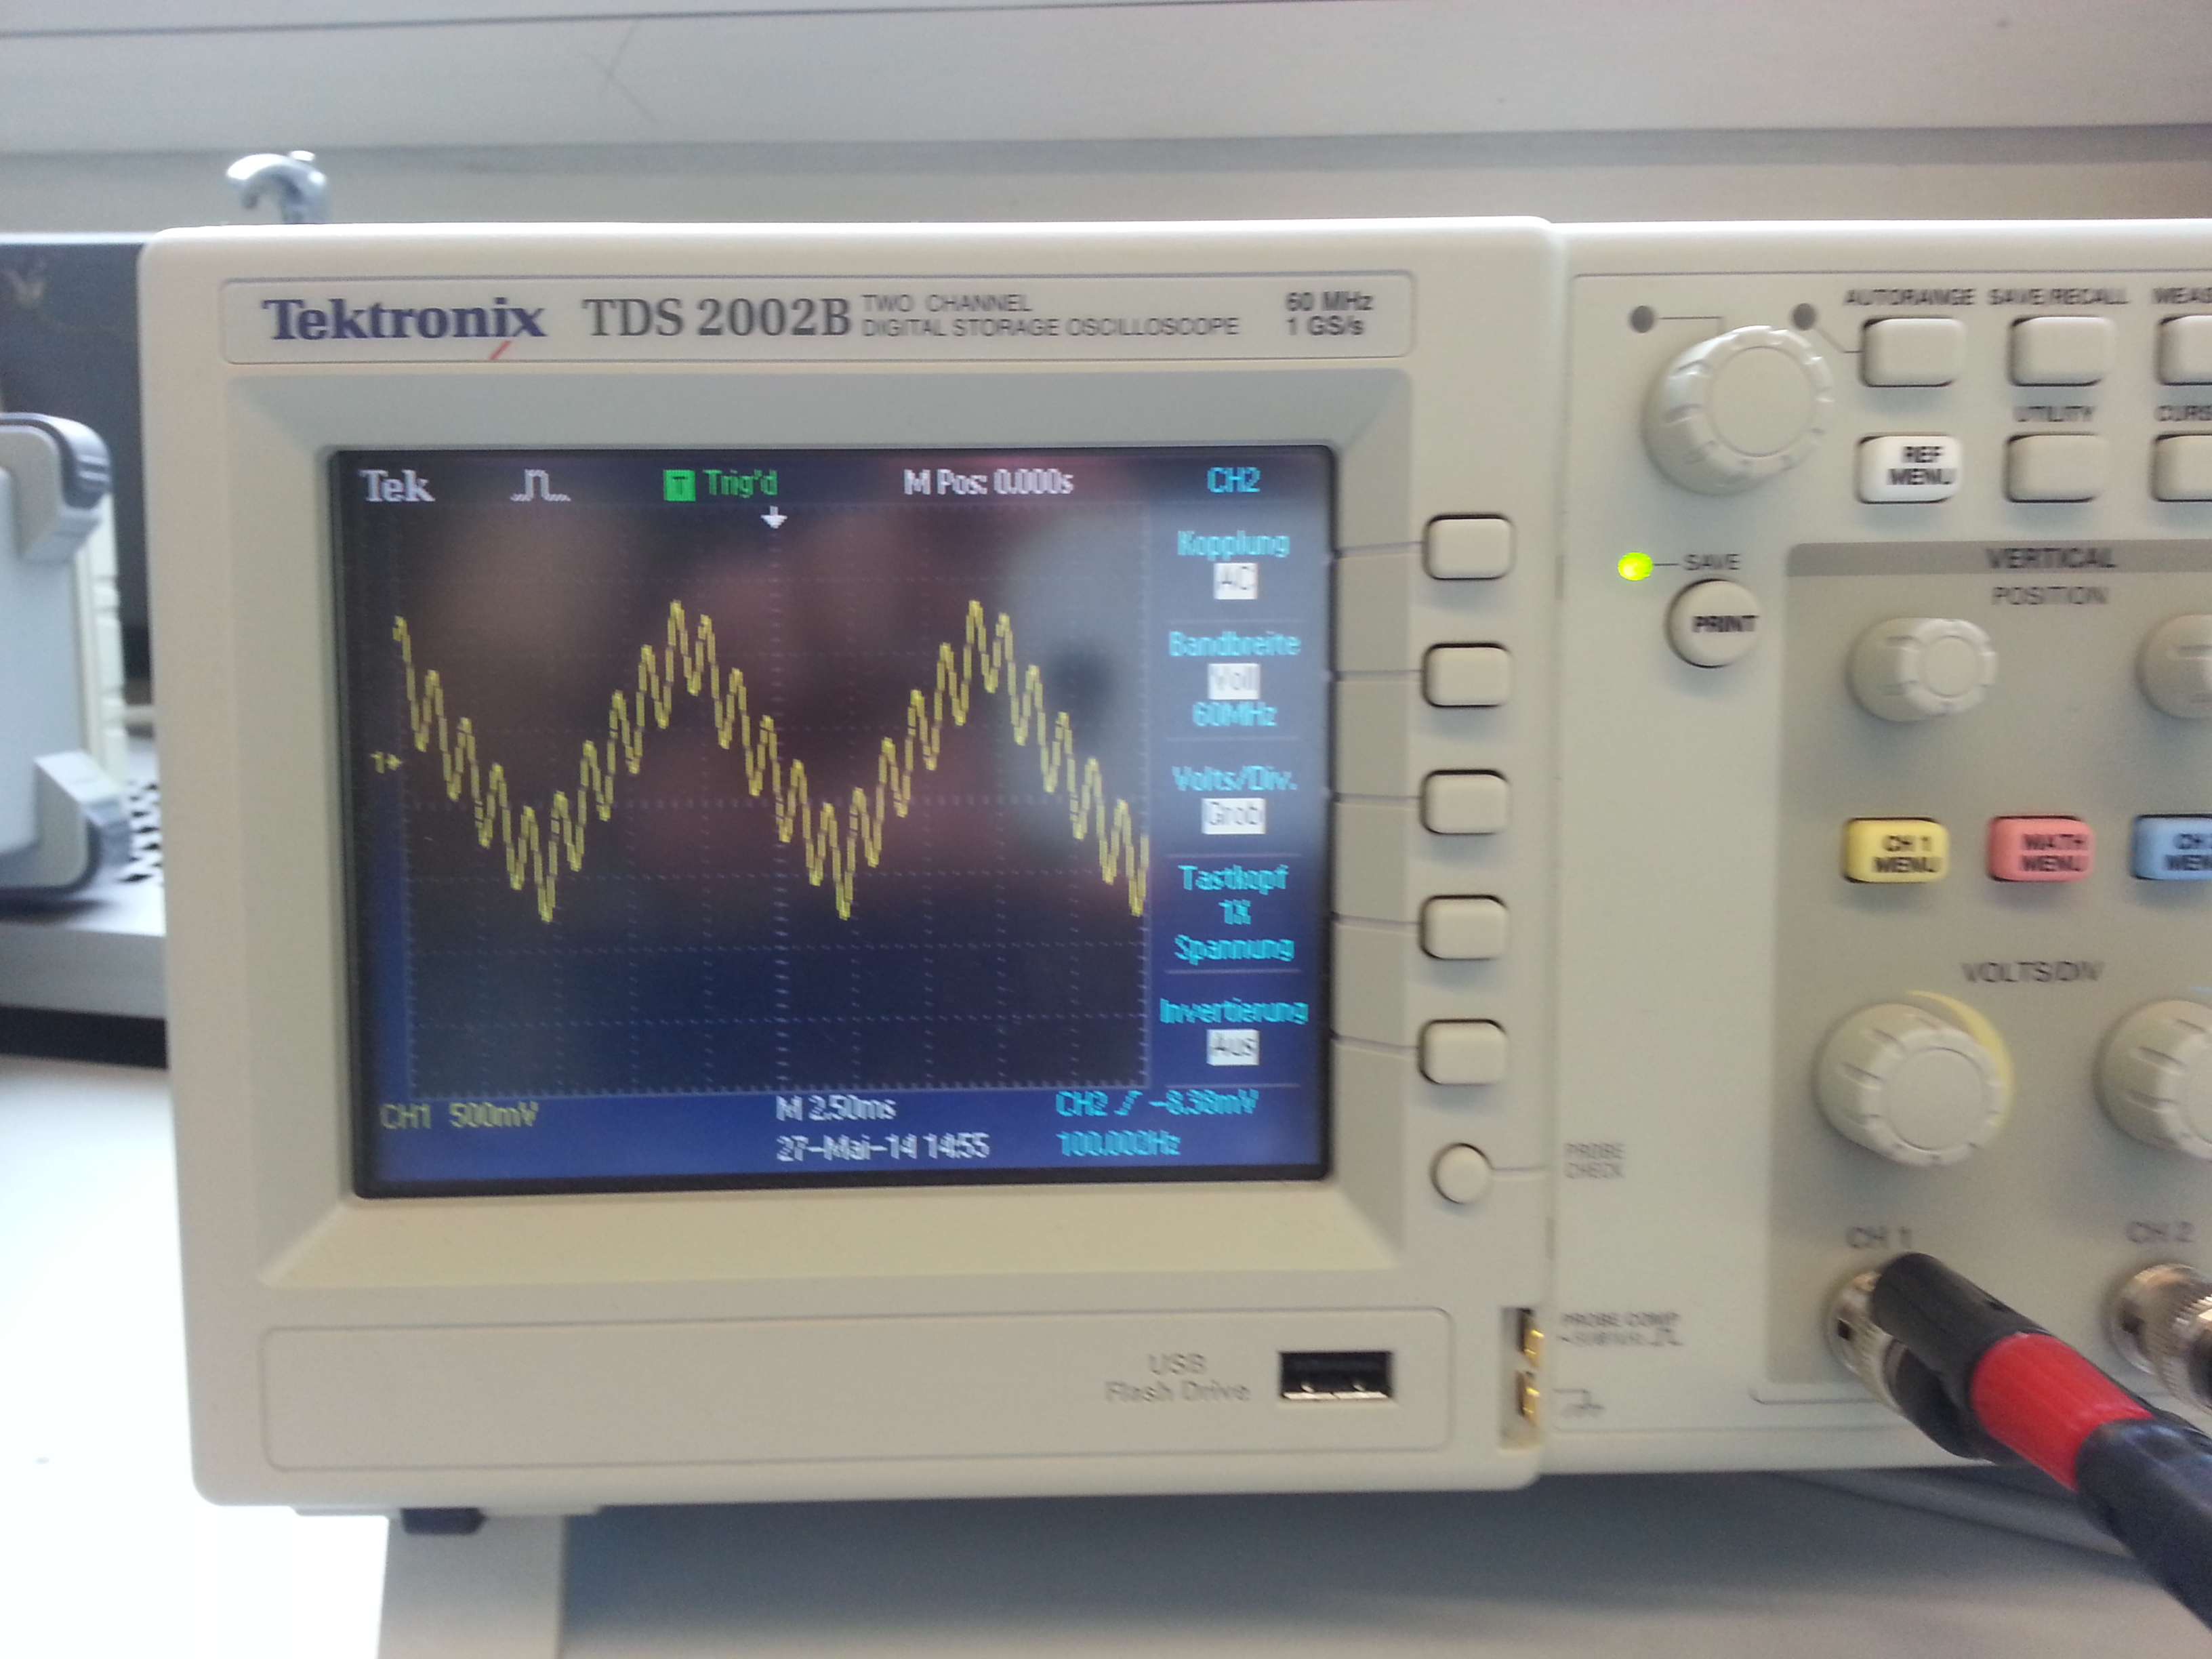
\includegraphics[scale=.08]{bilder/aufgabe_3_2_2.jpg} 
\caption{Oszilloskopbild der Addition von Sinus- und Dreiecksspannung}
\end{figure}

\subsection{Integrierer}

Ersetzt man in der invertierenden Grundschaltung einen der Widerstände durch einen Kondensator, so erhält man einen Integrierer bzw. Differenzierer. Wie in der Vorbereitung erläutert wurde ein Integrierer aufgebaut und dann dessen Funktionsweise anhand verschiedener Eingangssignale getestet.\\
Wie auf dem Oszilloskop zusehen ist, wurde das rechteckige Eingangssignal zu einem dreieckigen Ausgangssignal integriert. Außerdem sieht man auch, dass das Vorzeichen beim integrieren umgekehrt wurde, da wir ja von der invertierenden Grundschaltung ausgegangen sind.

\begin{figure}[H]
\centering
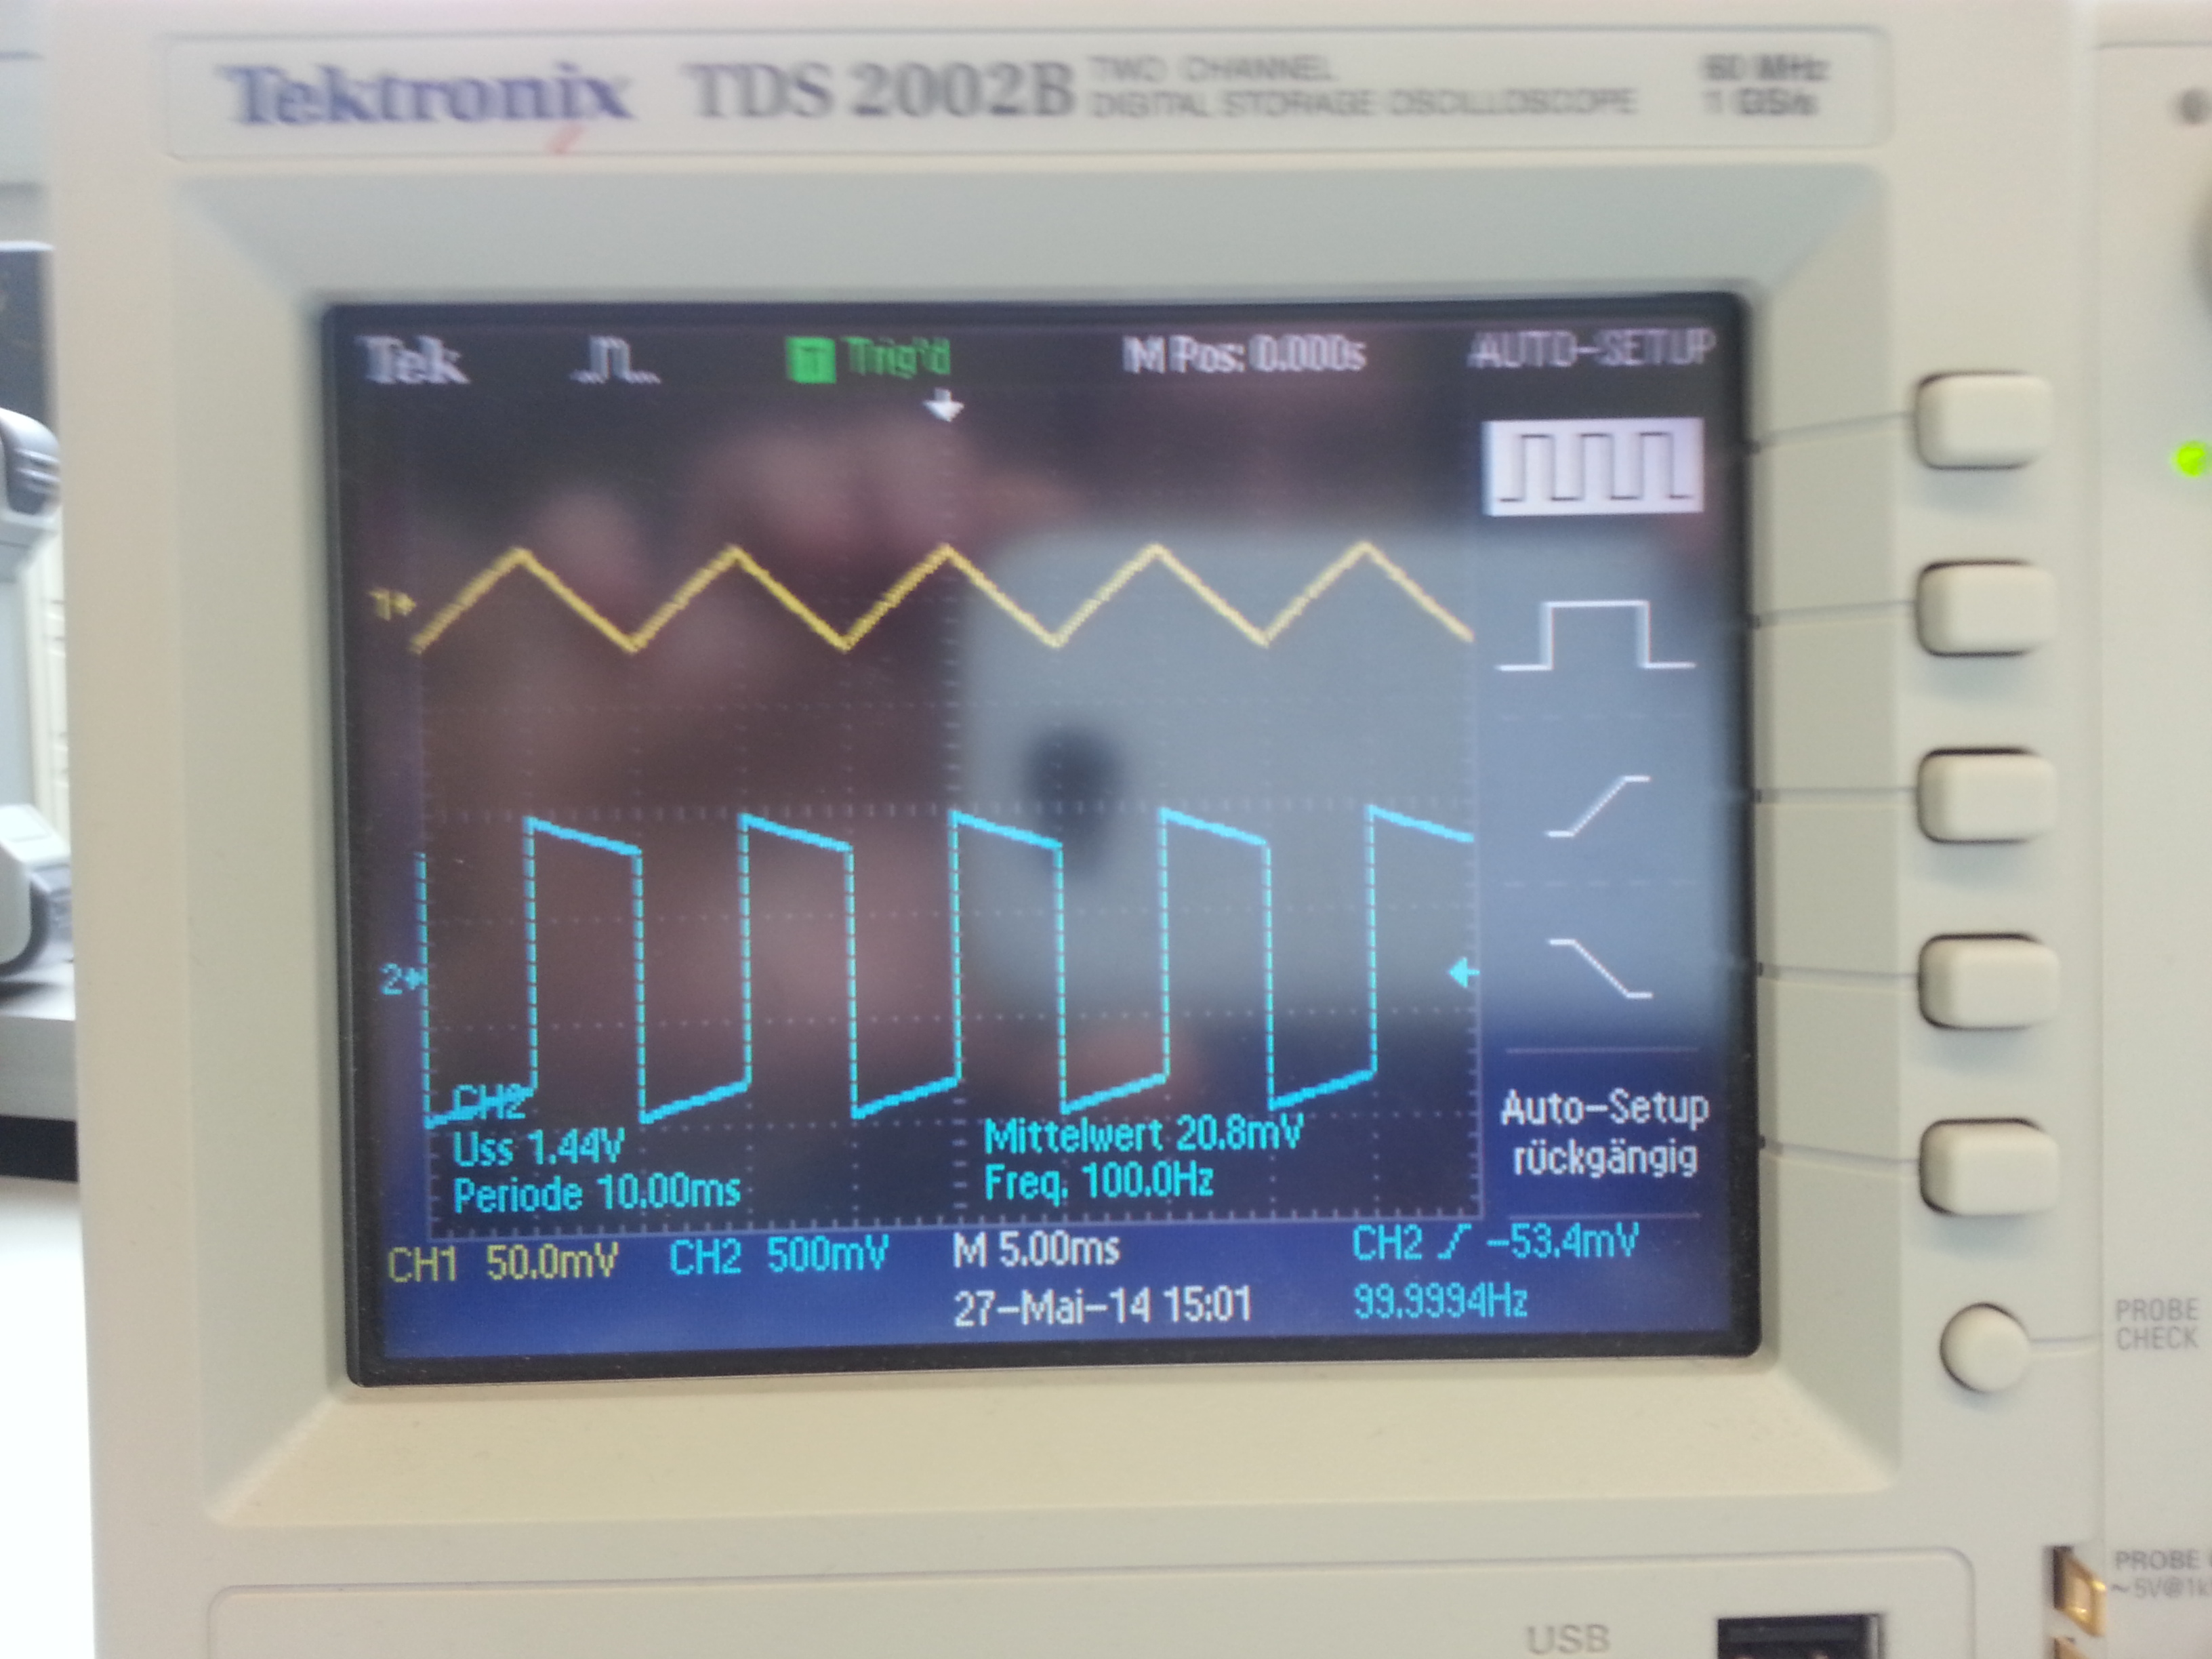
\includegraphics[scale=.08]{bilder/aufgabe_3_3_1.jpg} 
\caption{Oszilloskopbild der Integration der Rechtecksspannung}
\end{figure}

Die Dreiecksspannung wird im Integrierer wie erwartet zu einer aus hyperbelförmigen Spannung. Auch hierbei wurde das Vorzeichen wieder invertiert.

\begin{figure}[H]
\centering
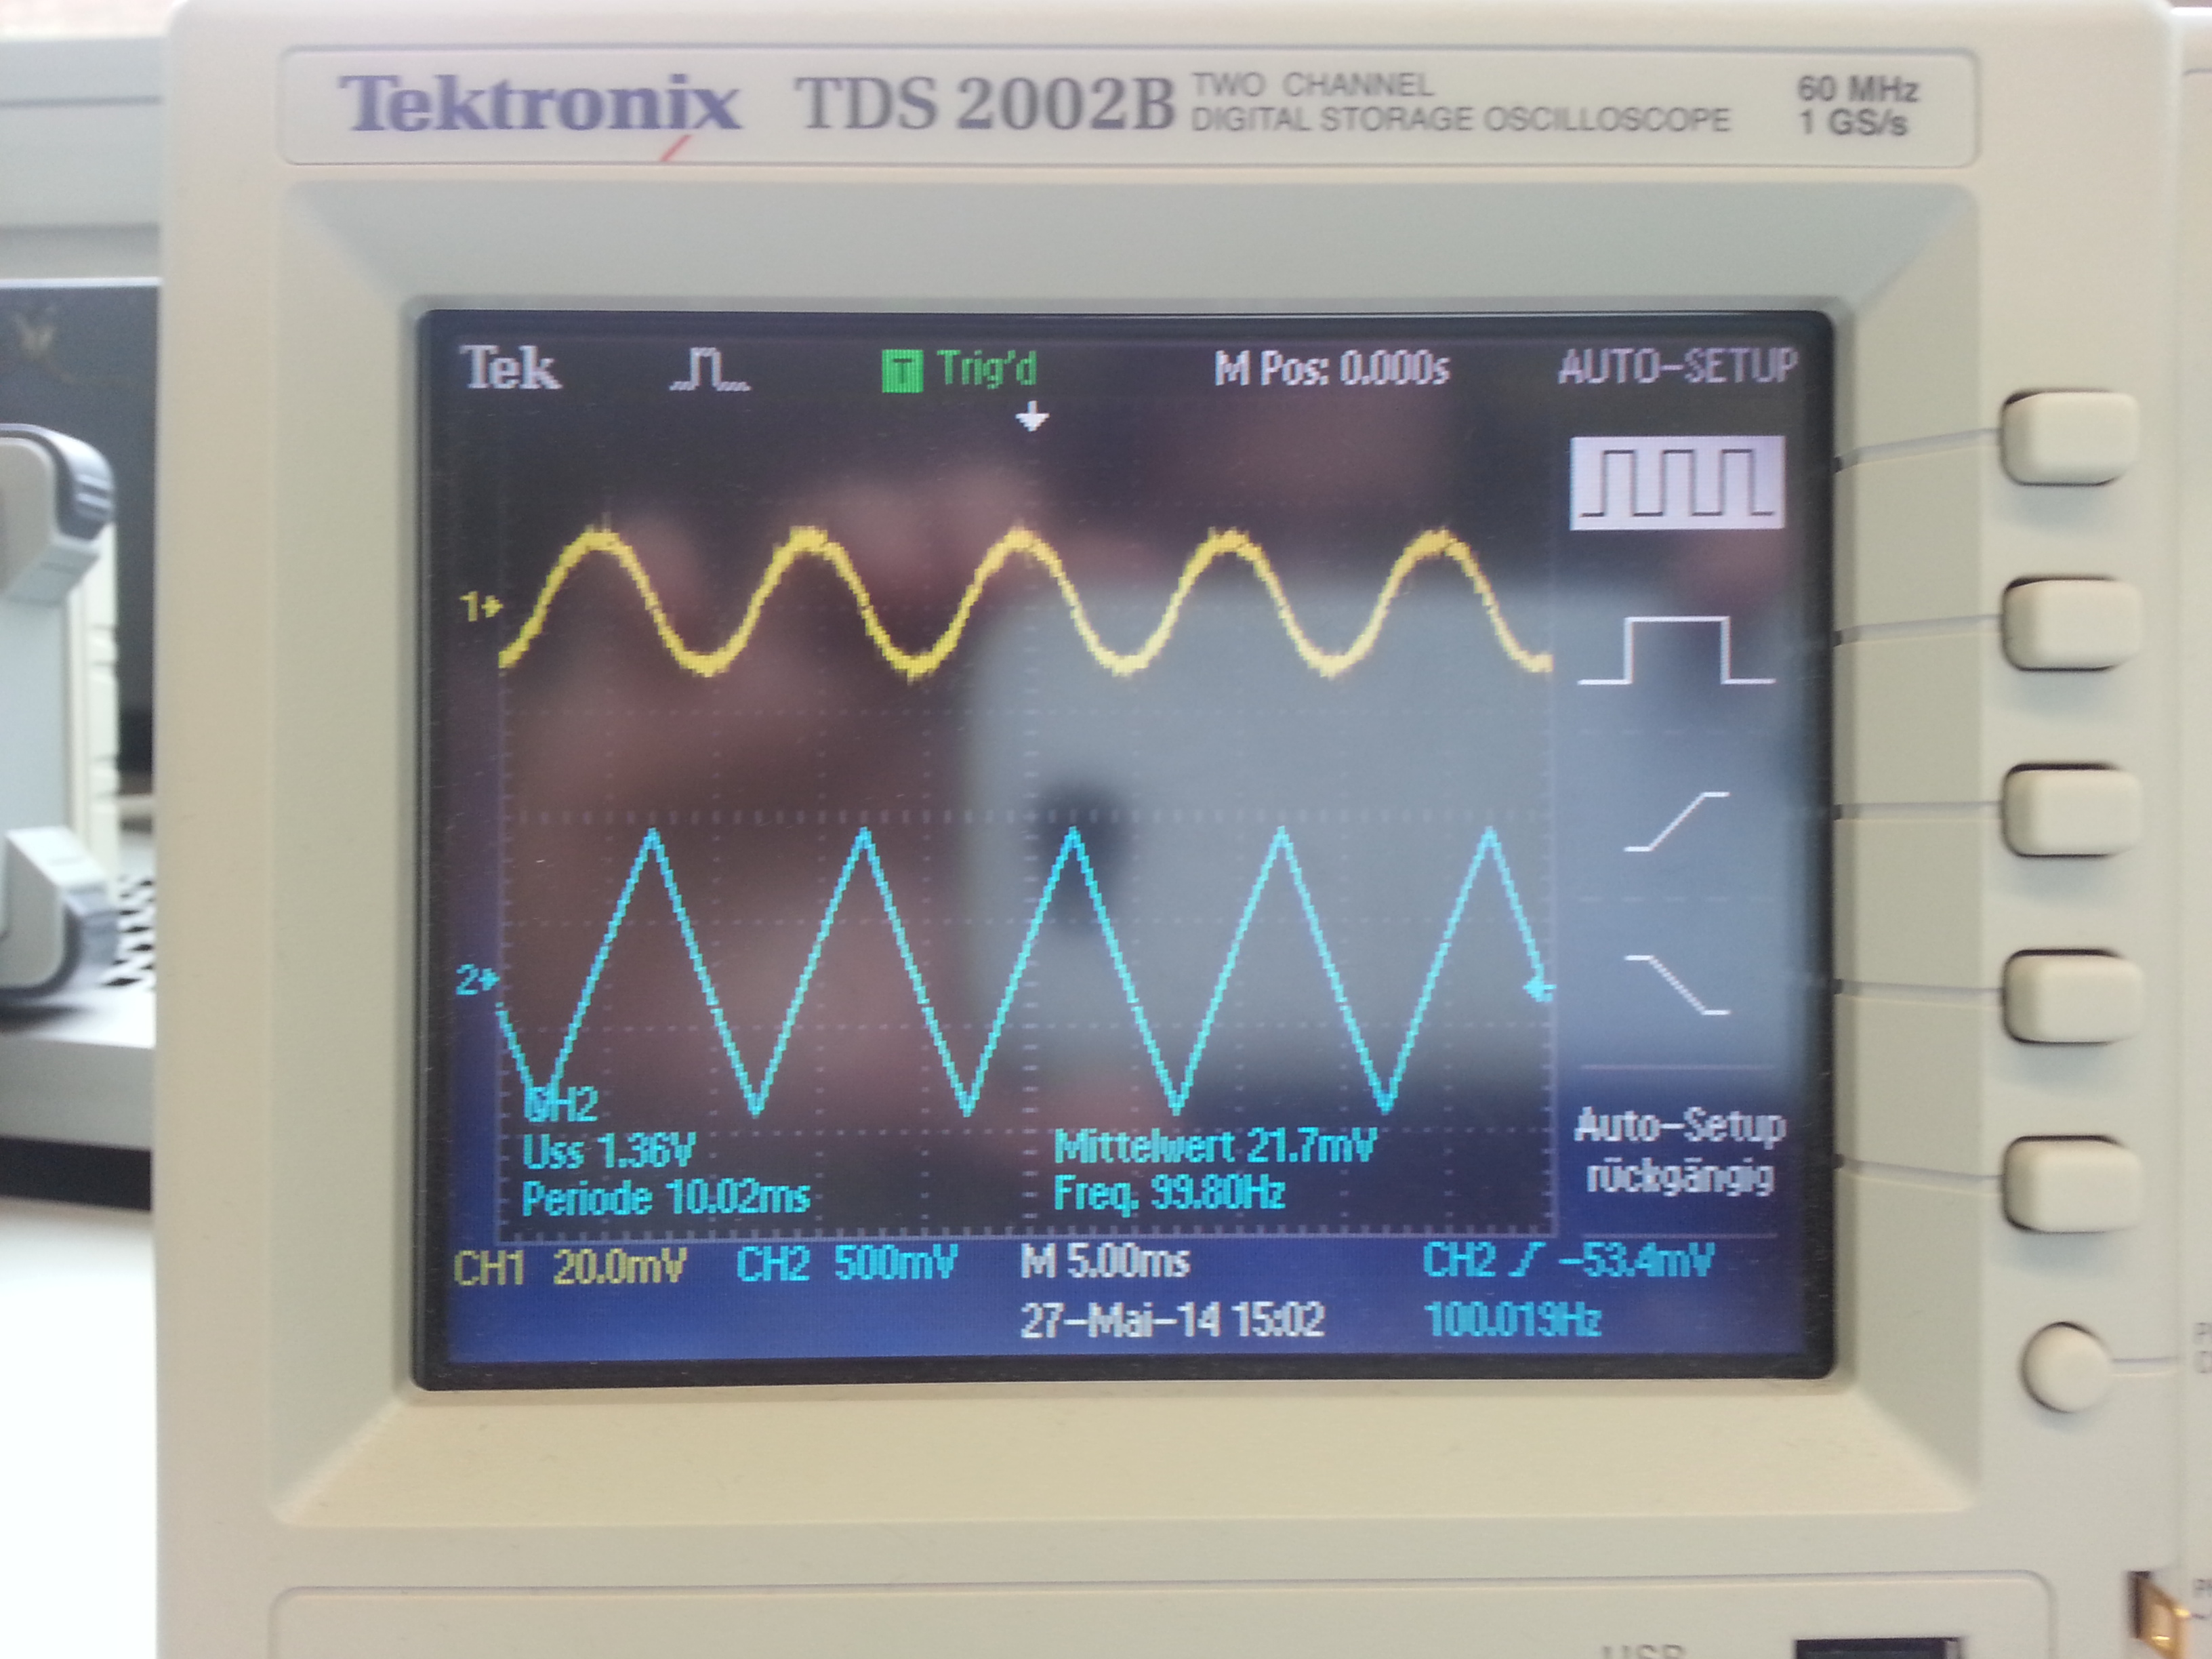
\includegraphics[scale=.08]{bilder/aufgabe_3_3_2.jpg} 
\caption{Oszilloskopbild der Integration der Dreiecksspannung}
\end{figure}

\subsection{Differenzierer}

Der Differenzierer ist ähnlich aufgebaut wie der Integrierer, wobei hier der Widerstand in der Zuleitung durch einen Kondensator ersetzt wird (siehe Vorbereitung). Die Funktionsweise des Differenzierers haben wir wiederum an Rechtecks- und Dreiecksspannung verdeutlicht.\\
Da wir ja bereits in der vorherigen Aufgabe beim Integrieren der Rechtecksspannung, eine Dreiecksspannung erhielten, war klar, dass man beim Differenzieren der Dreiecksspannung nun auch ein rechteckiges Signal erhalten sollte. Dies war in der Tat auch zu beobachten.

\begin{figure}[H]
\centering
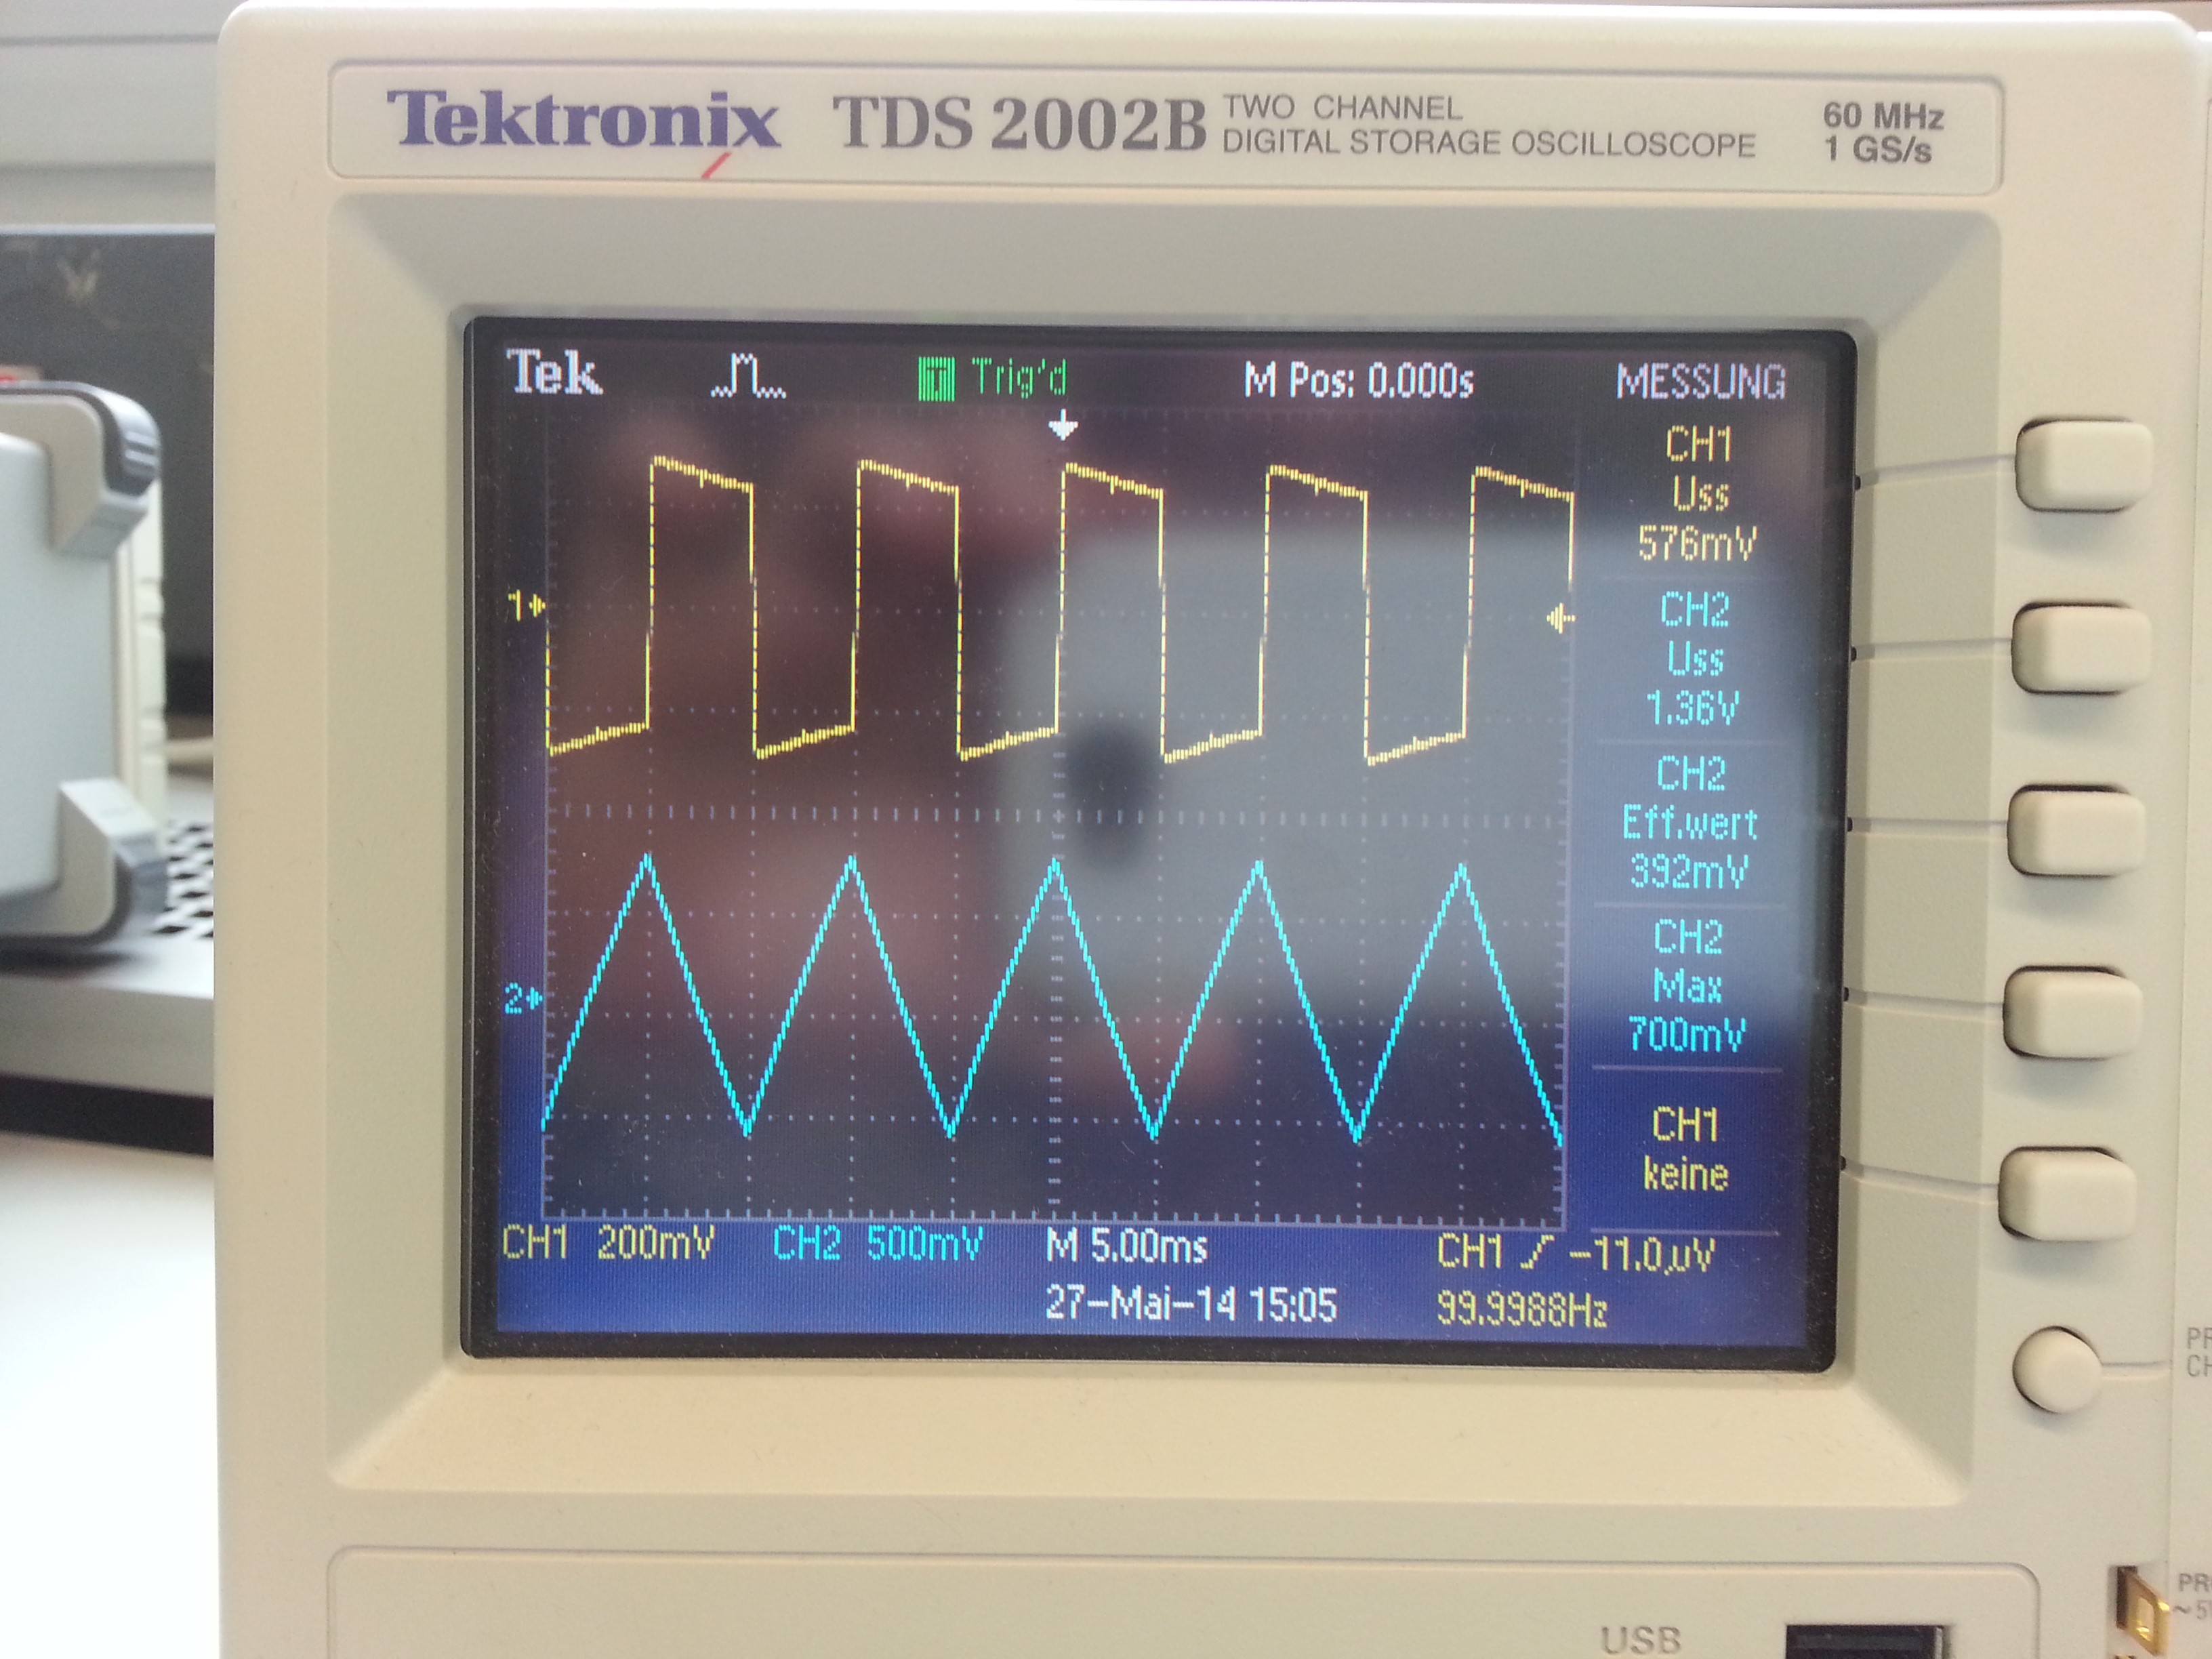
\includegraphics[scale=.08]{bilder/aufgabe_3_4_1.jpg} 
\caption{Oszilloskopbild der Differenzierung der Dreiecksspannung}
\end{figure}

Das Differenzieren des rechteckigen Eingangssignals lieferte und eine Art Deltapeaks als Ausgangssignal, da die Steigung des Rechtecks an den Seiten unendlich und sonst Null ist.

\begin{figure}[H]
\centering
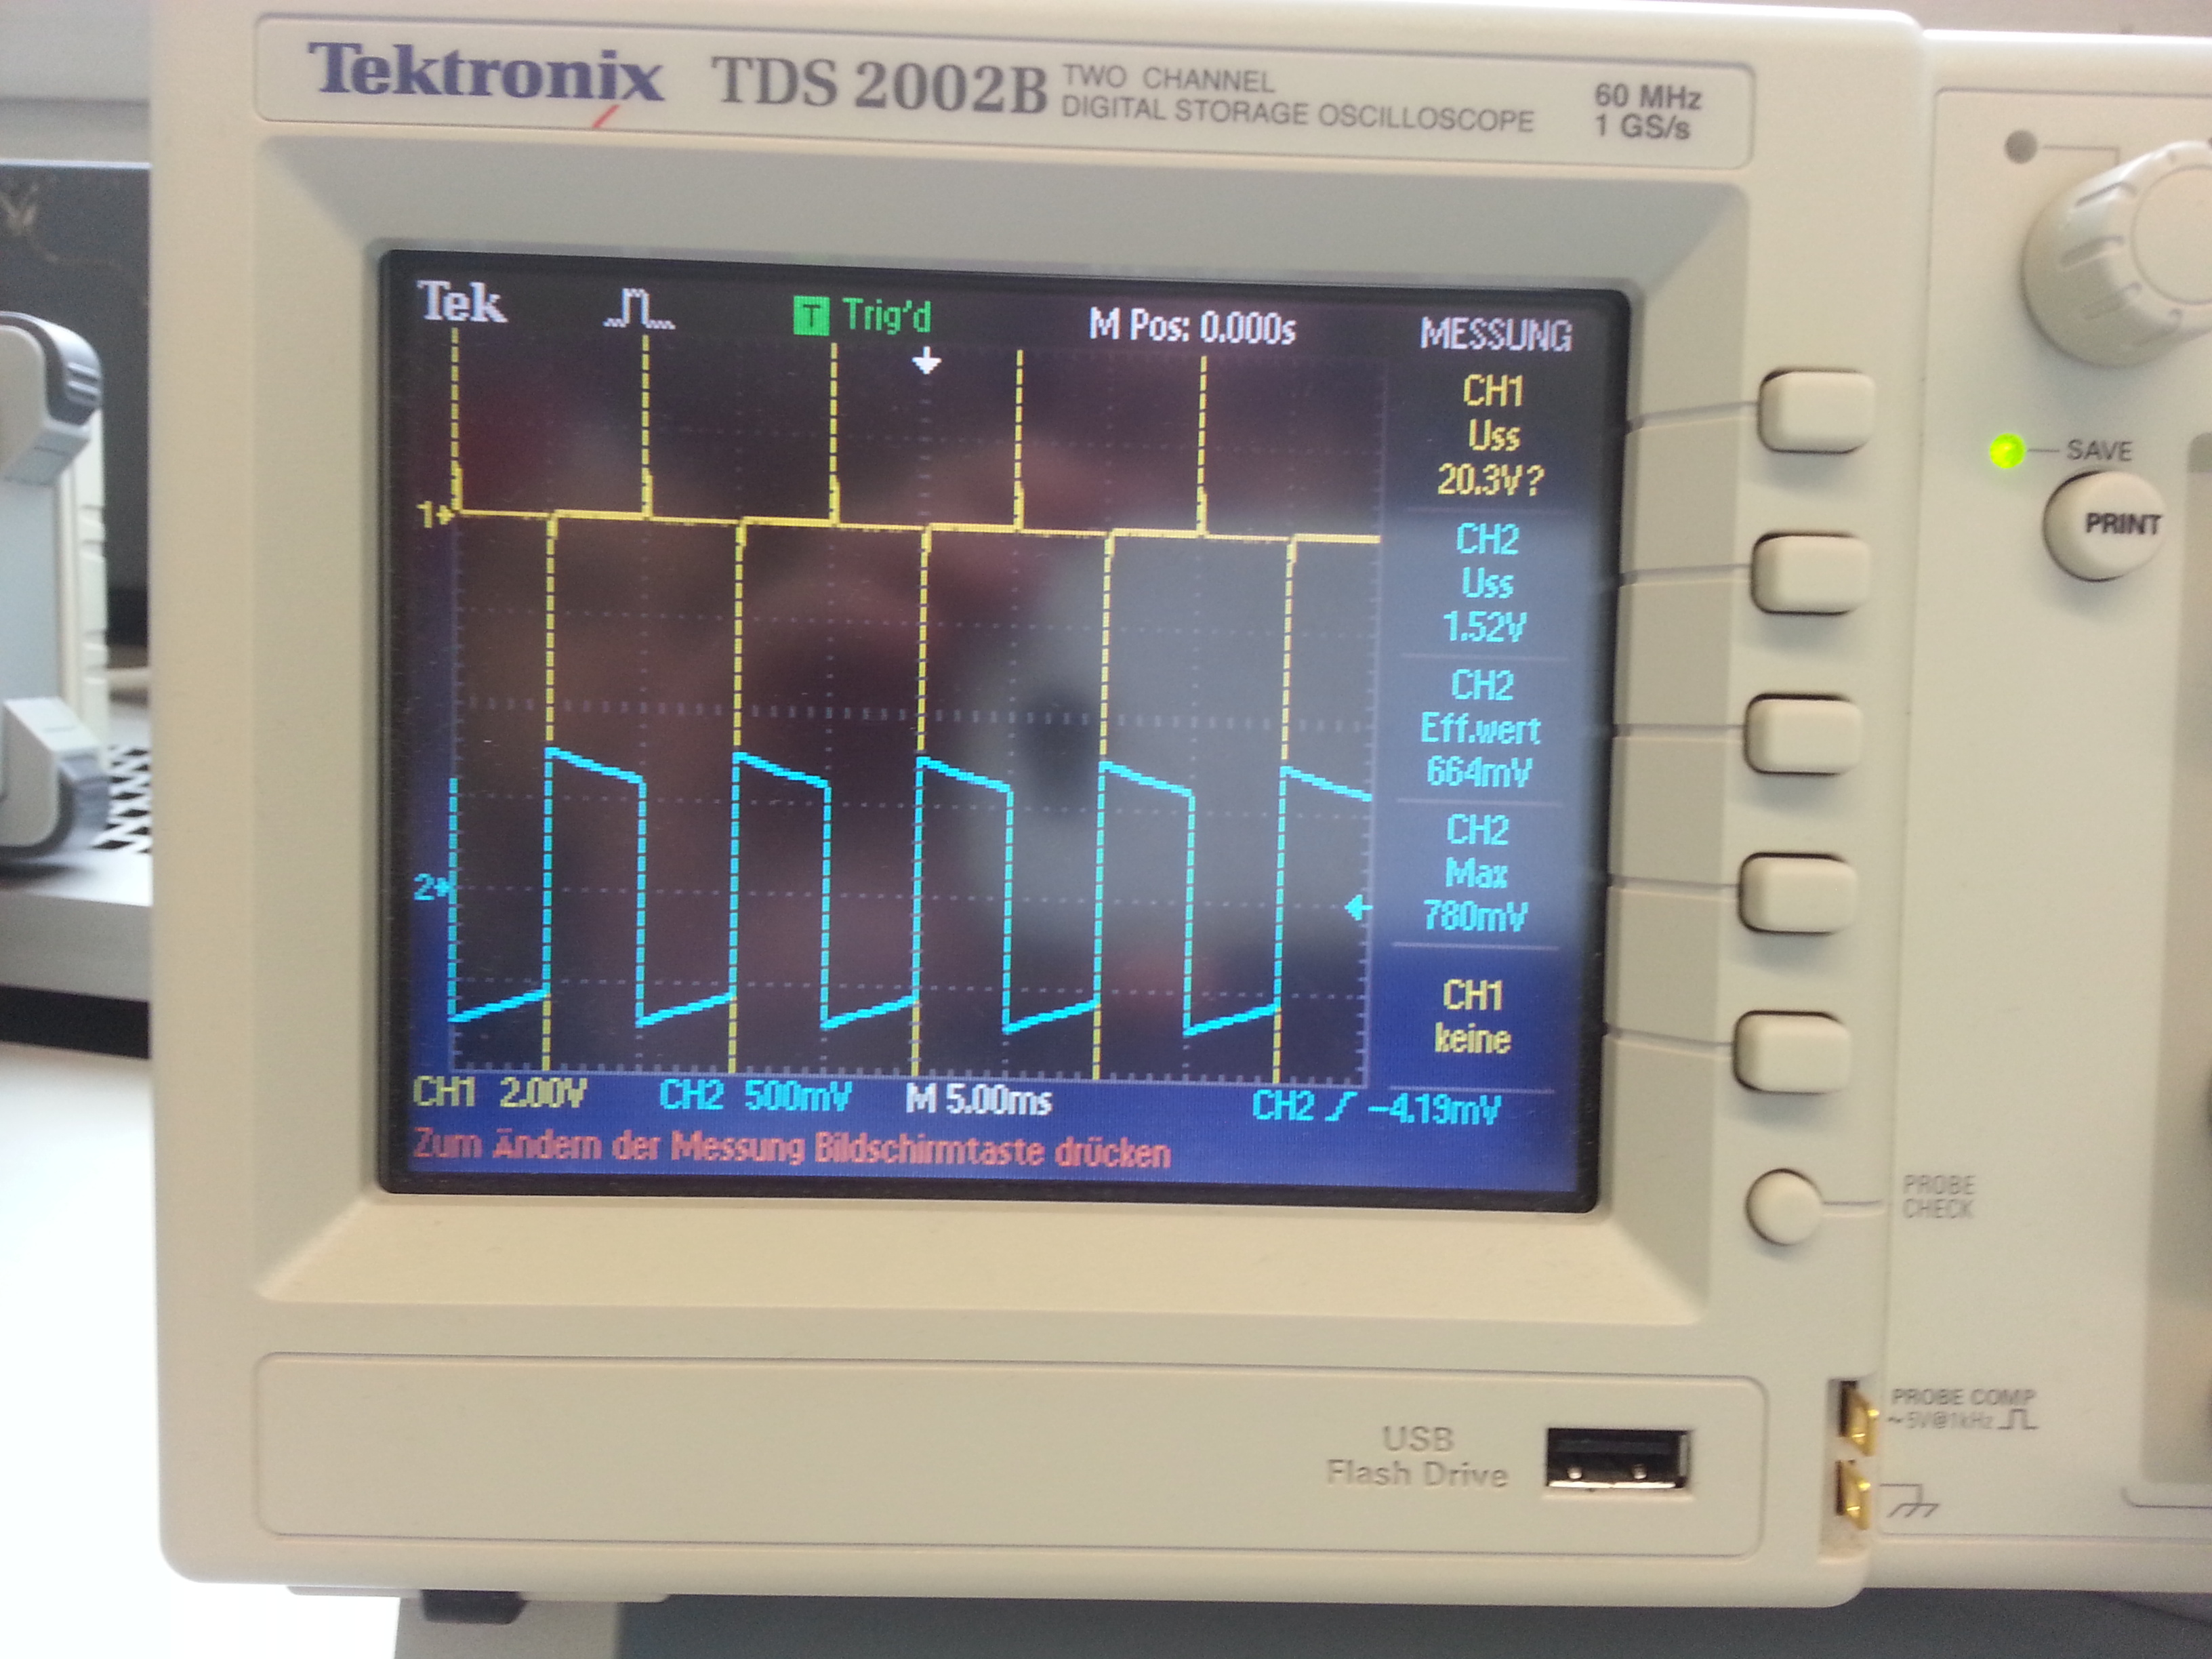
\includegraphics[scale=.08]{bilder/aufgabe_3_4_2.jpg} 
\caption{Oszilloskopbild der Differenzierung der Rechtecksspannung}
\end{figure}

\section{Komplexere Schaltungen}
\subsection{Idealer Einweggleichrichter}

In der Vorbereitung wurde bereits erwähnt, dass ein einfacher Diodengleichrichter den Nachteil hat, dass an den Dioden die Diodenknickspannung abfällt und deshalb ein ''zu kleines'' Ausgangssignal ausgegeben wird. Baut man die Schaltung einen Operationsverstärker mit ein, welcher diese Diodenknickspannung ausgleichen kann, so erhält man eine komplette Halbwelle als Ausgangssignal.

\begin{figure}[H]
\centering
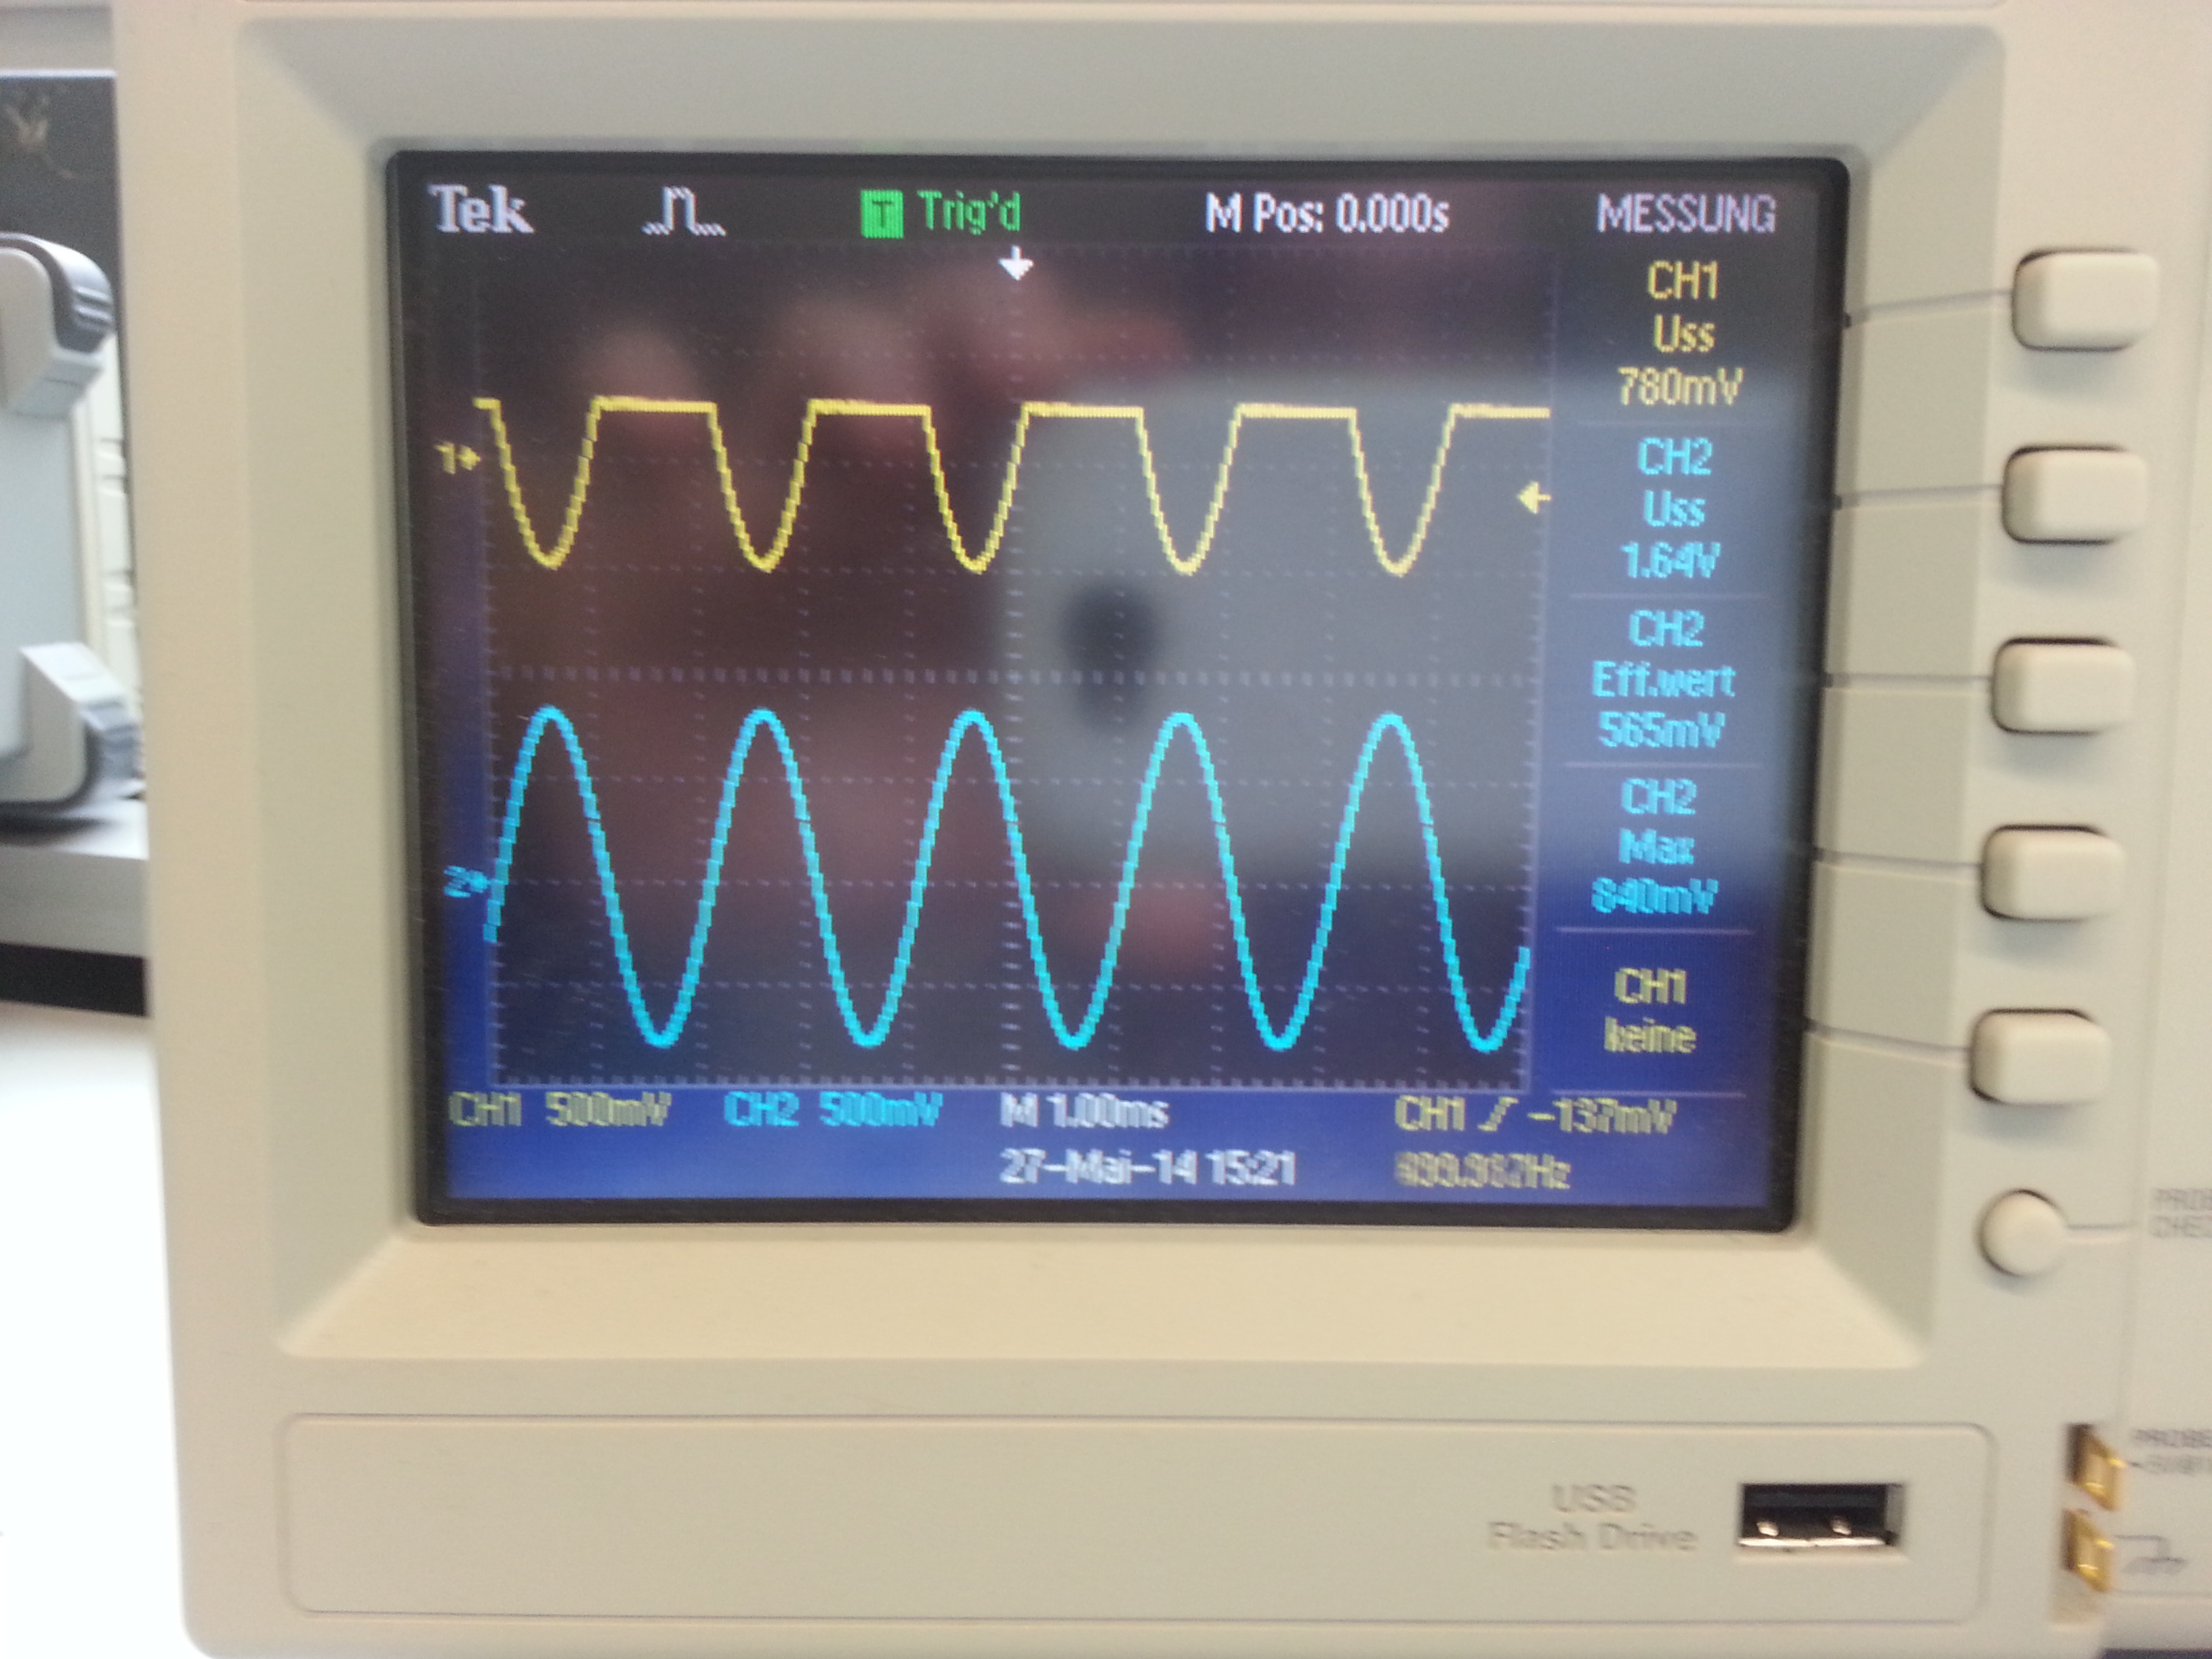
\includegraphics[scale=.08]{bilder/aufgabe_4_1_1.jpg} 
\caption{Idealer Einweggleichrichter mit Operationsverstärker}
\end{figure}

\begin{figure}[H]
\centering
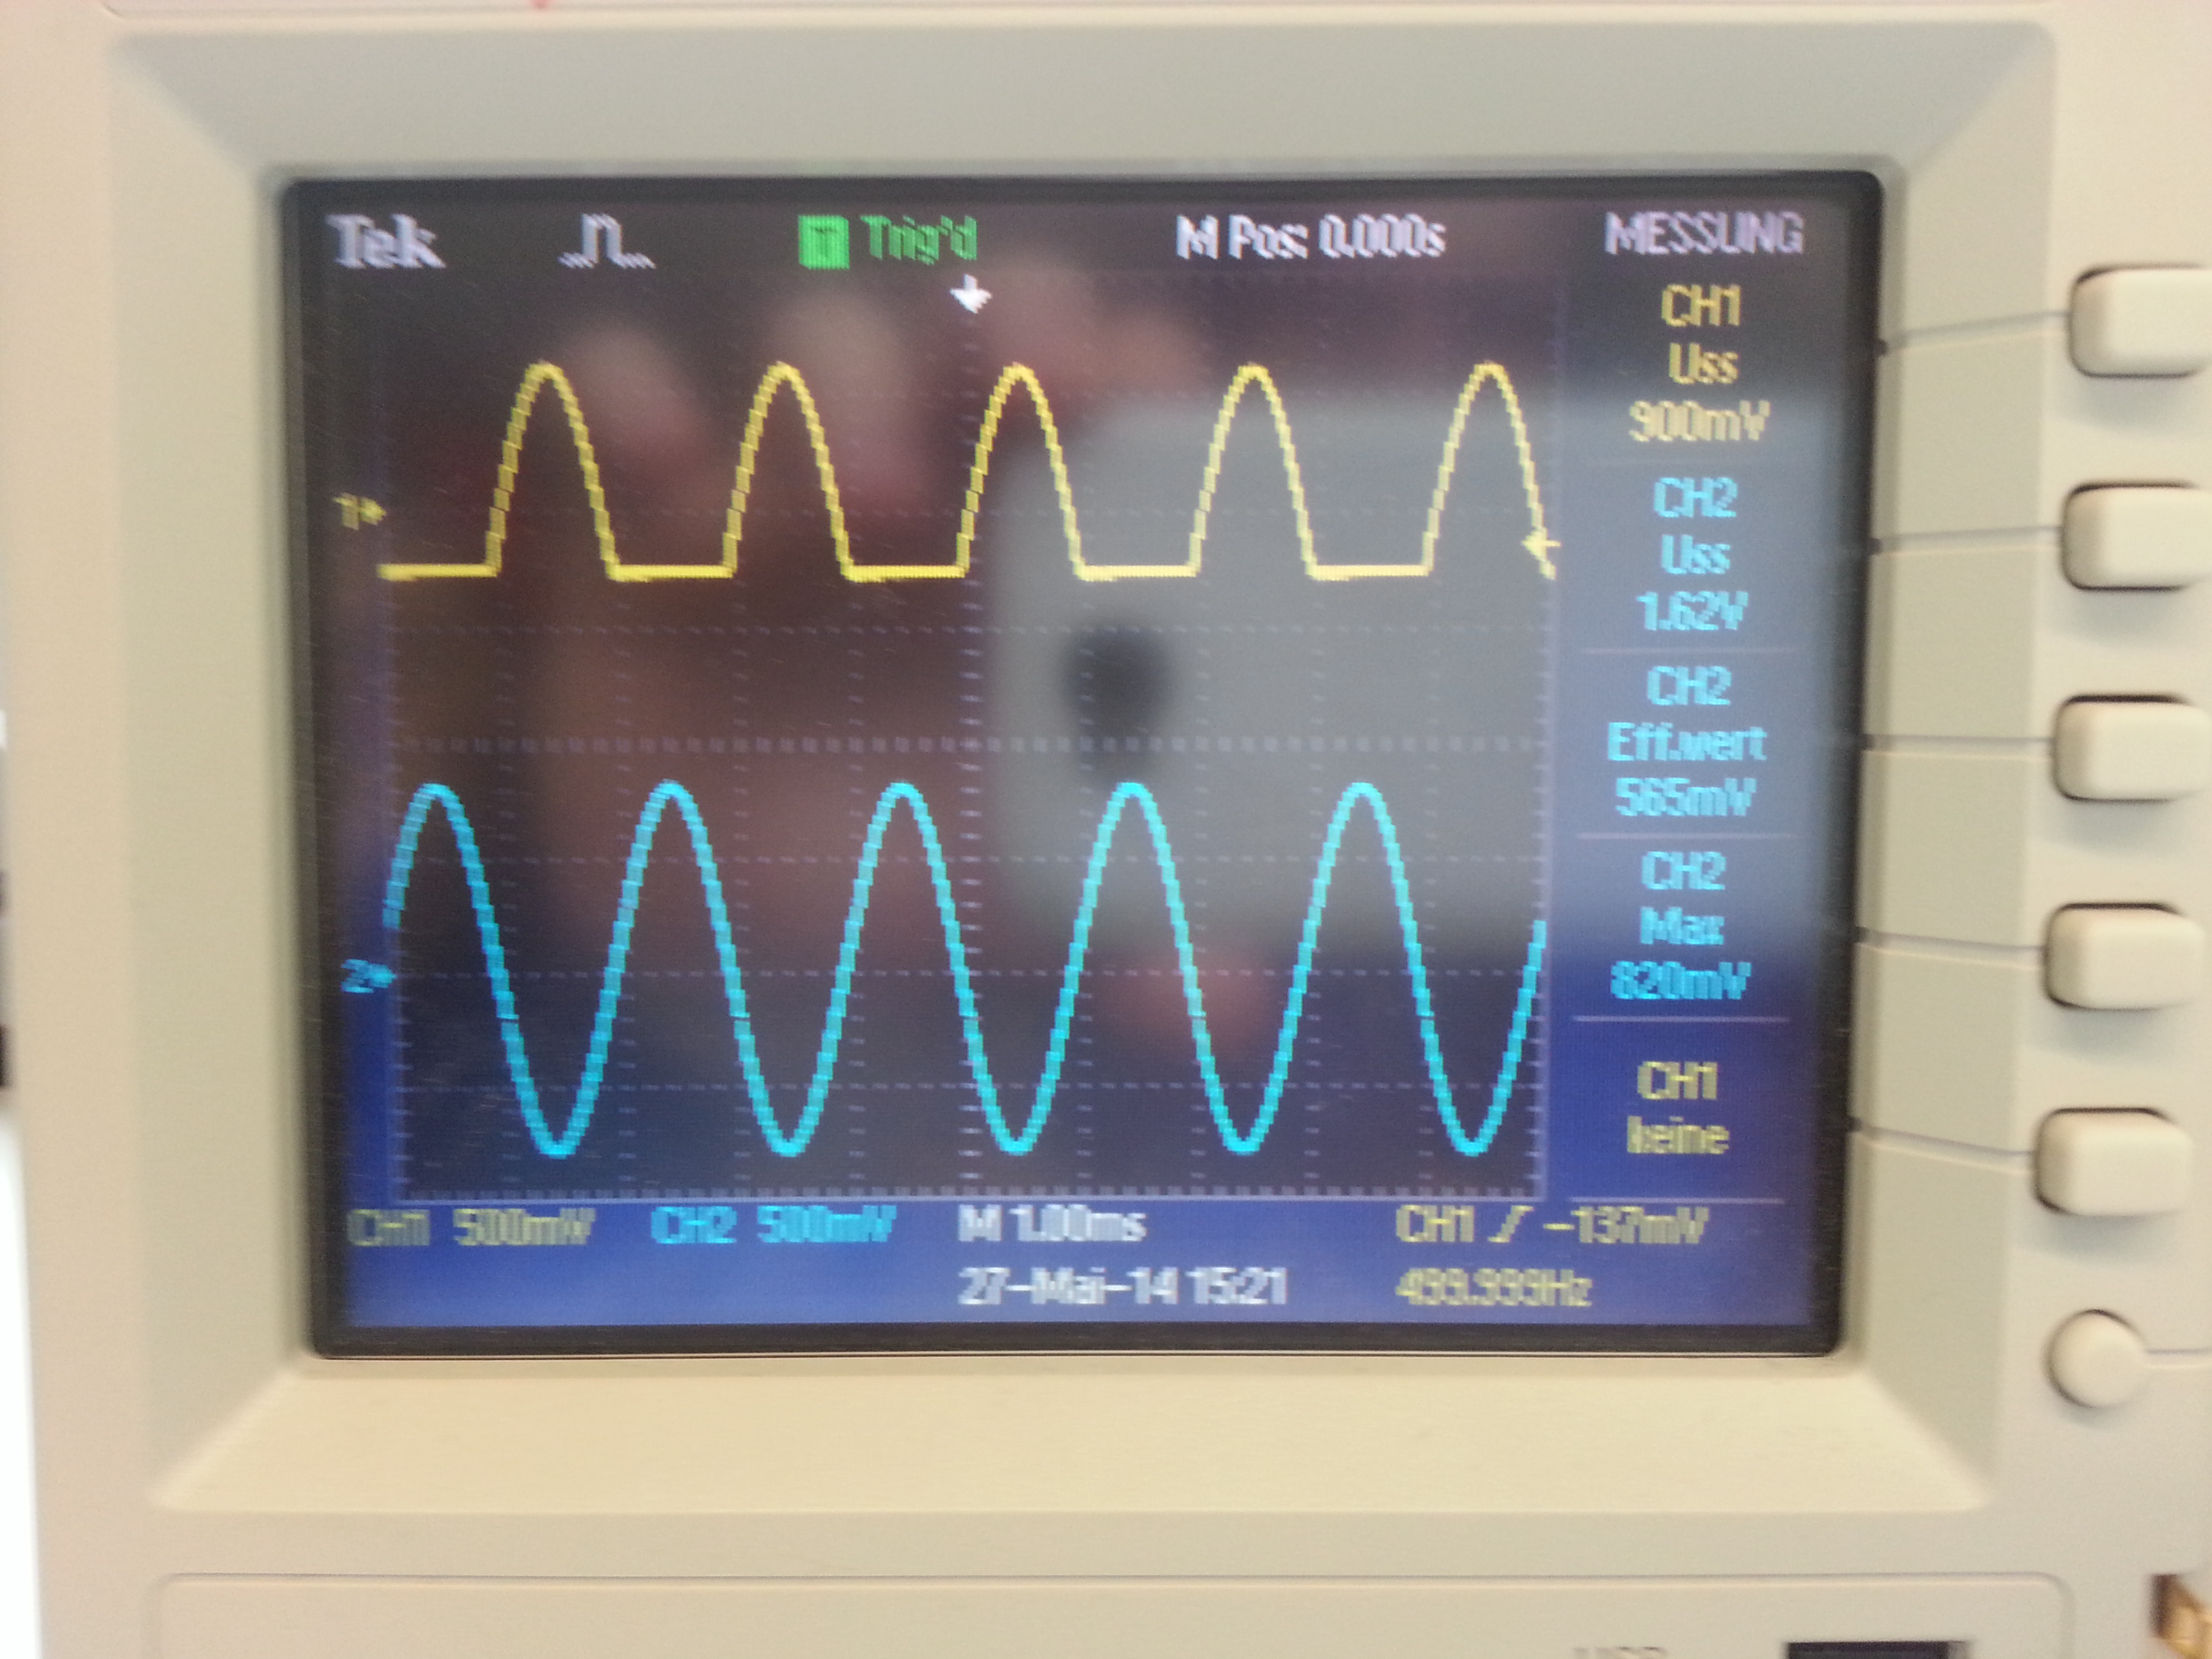
\includegraphics[scale=.08]{bilder/aufgabe_4_1_2.jpg} 
\caption{Idealer Einweggleichrichter mit Operationsverstärker}
\end{figure}

Die Abbildungen zeigen jeweils ein Ausgangssignal der Schaltung. Wie leicht zu erkennen ist, wird genau die invertierte Halbwelle des Eingangssignal ausgegeben. 

\begin{figure}[H]
\centering
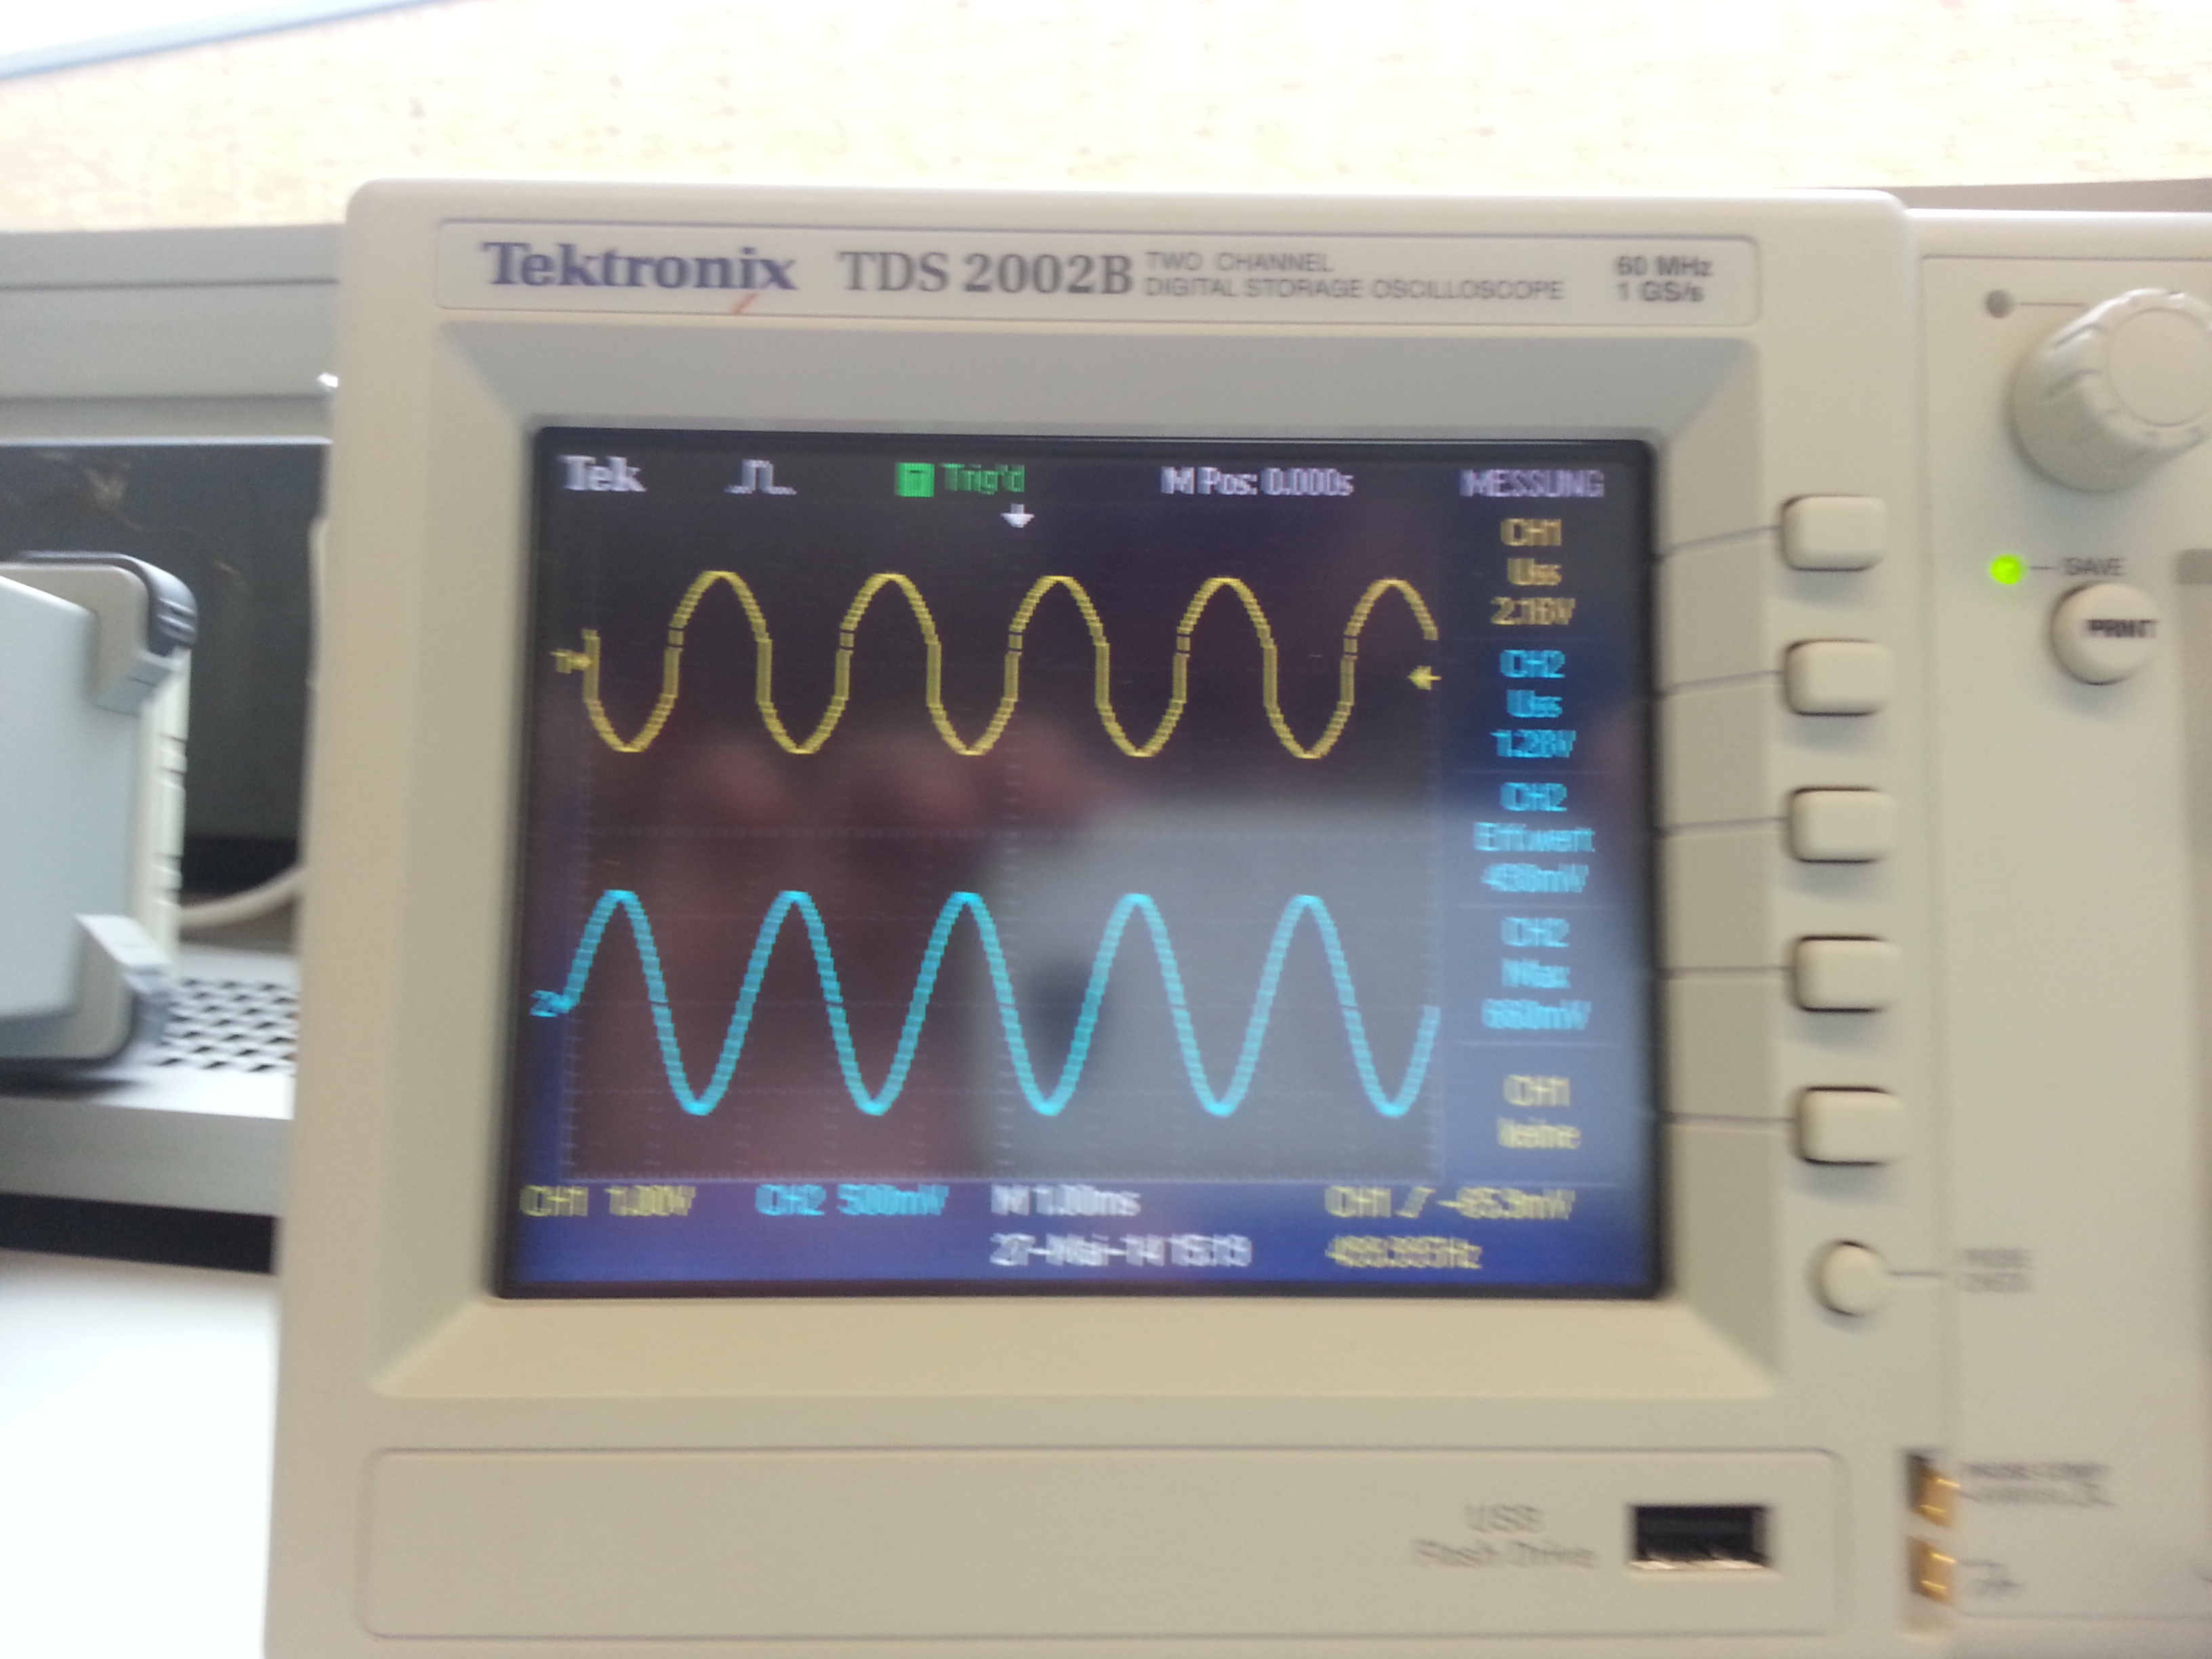
\includegraphics[scale=.08]{bilder/aufgabe_4_1_3.jpg} 
\caption{Idealer Einweggleichrichter mit Operationsverstärker}
\end{figure}

In der letzten Abbildung sieht man das Signal am Ausgang des Operationsverstärkers. Das Signal hat bei jedem Vorzeichenwechsel eine Sprung, der gerade der doppelten Diodenknickspannung entspricht.

\subsection{Generator für Dreiecks- und Rechteckssignale}

Man kann mit zwei Operationsvertärkern einen Generator für Dreiecks-und Rechtecksspanungen baen. Dazu wird ein OPV als Integrierer und ein OPV als Schmitt-Trigger verwendet. Der Schmitt-Trigger schlägt beim Umschalten immer zwischen der positiven und negativen Sättigungsspannung hin und her. Der Integrierer macht dann aus dem Signal ein Dreieckssignal und sorgt dafür, dass der Trigger umschaltete (siehe Vorbereitung). Die Funktionsweise wurde von uns überprüft und bestätigt.

\begin{figure}[H]
\centering
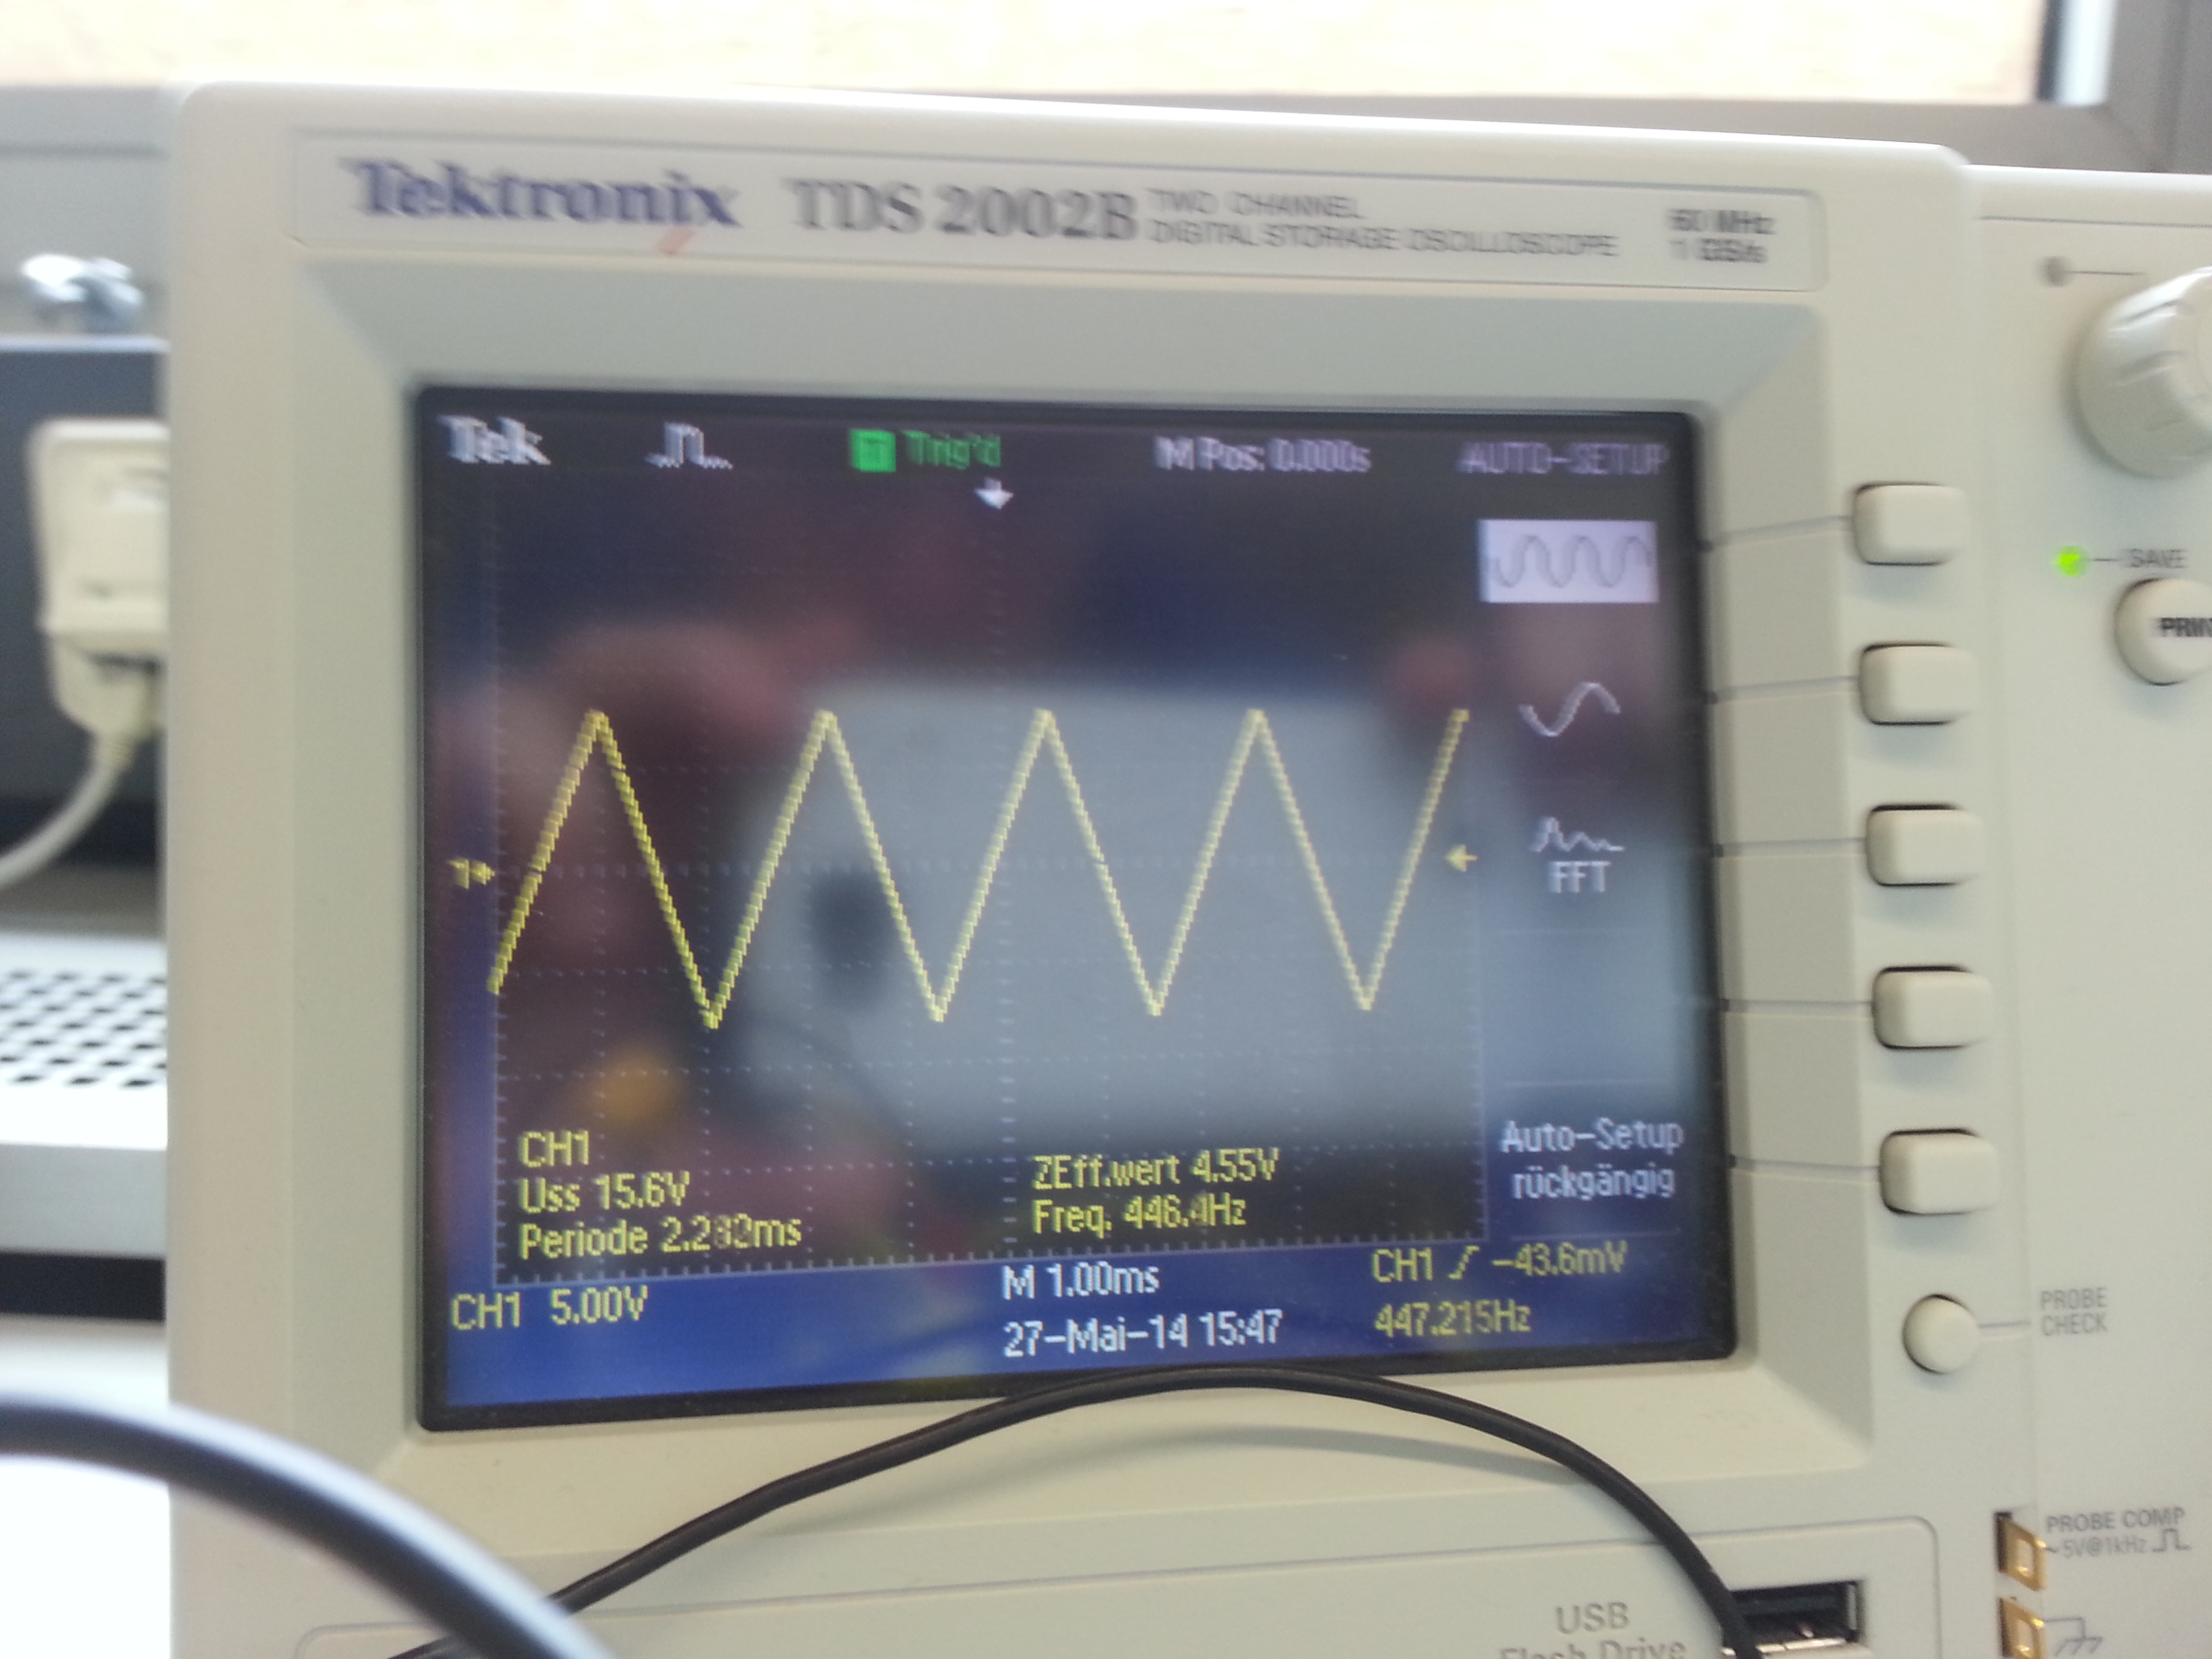
\includegraphics[scale=.08]{bilder/aufgabe_4_2_1.jpg} 
\caption{Generator: Dreieckssignal}
\end{figure}

\begin{figure}[H]
\centering
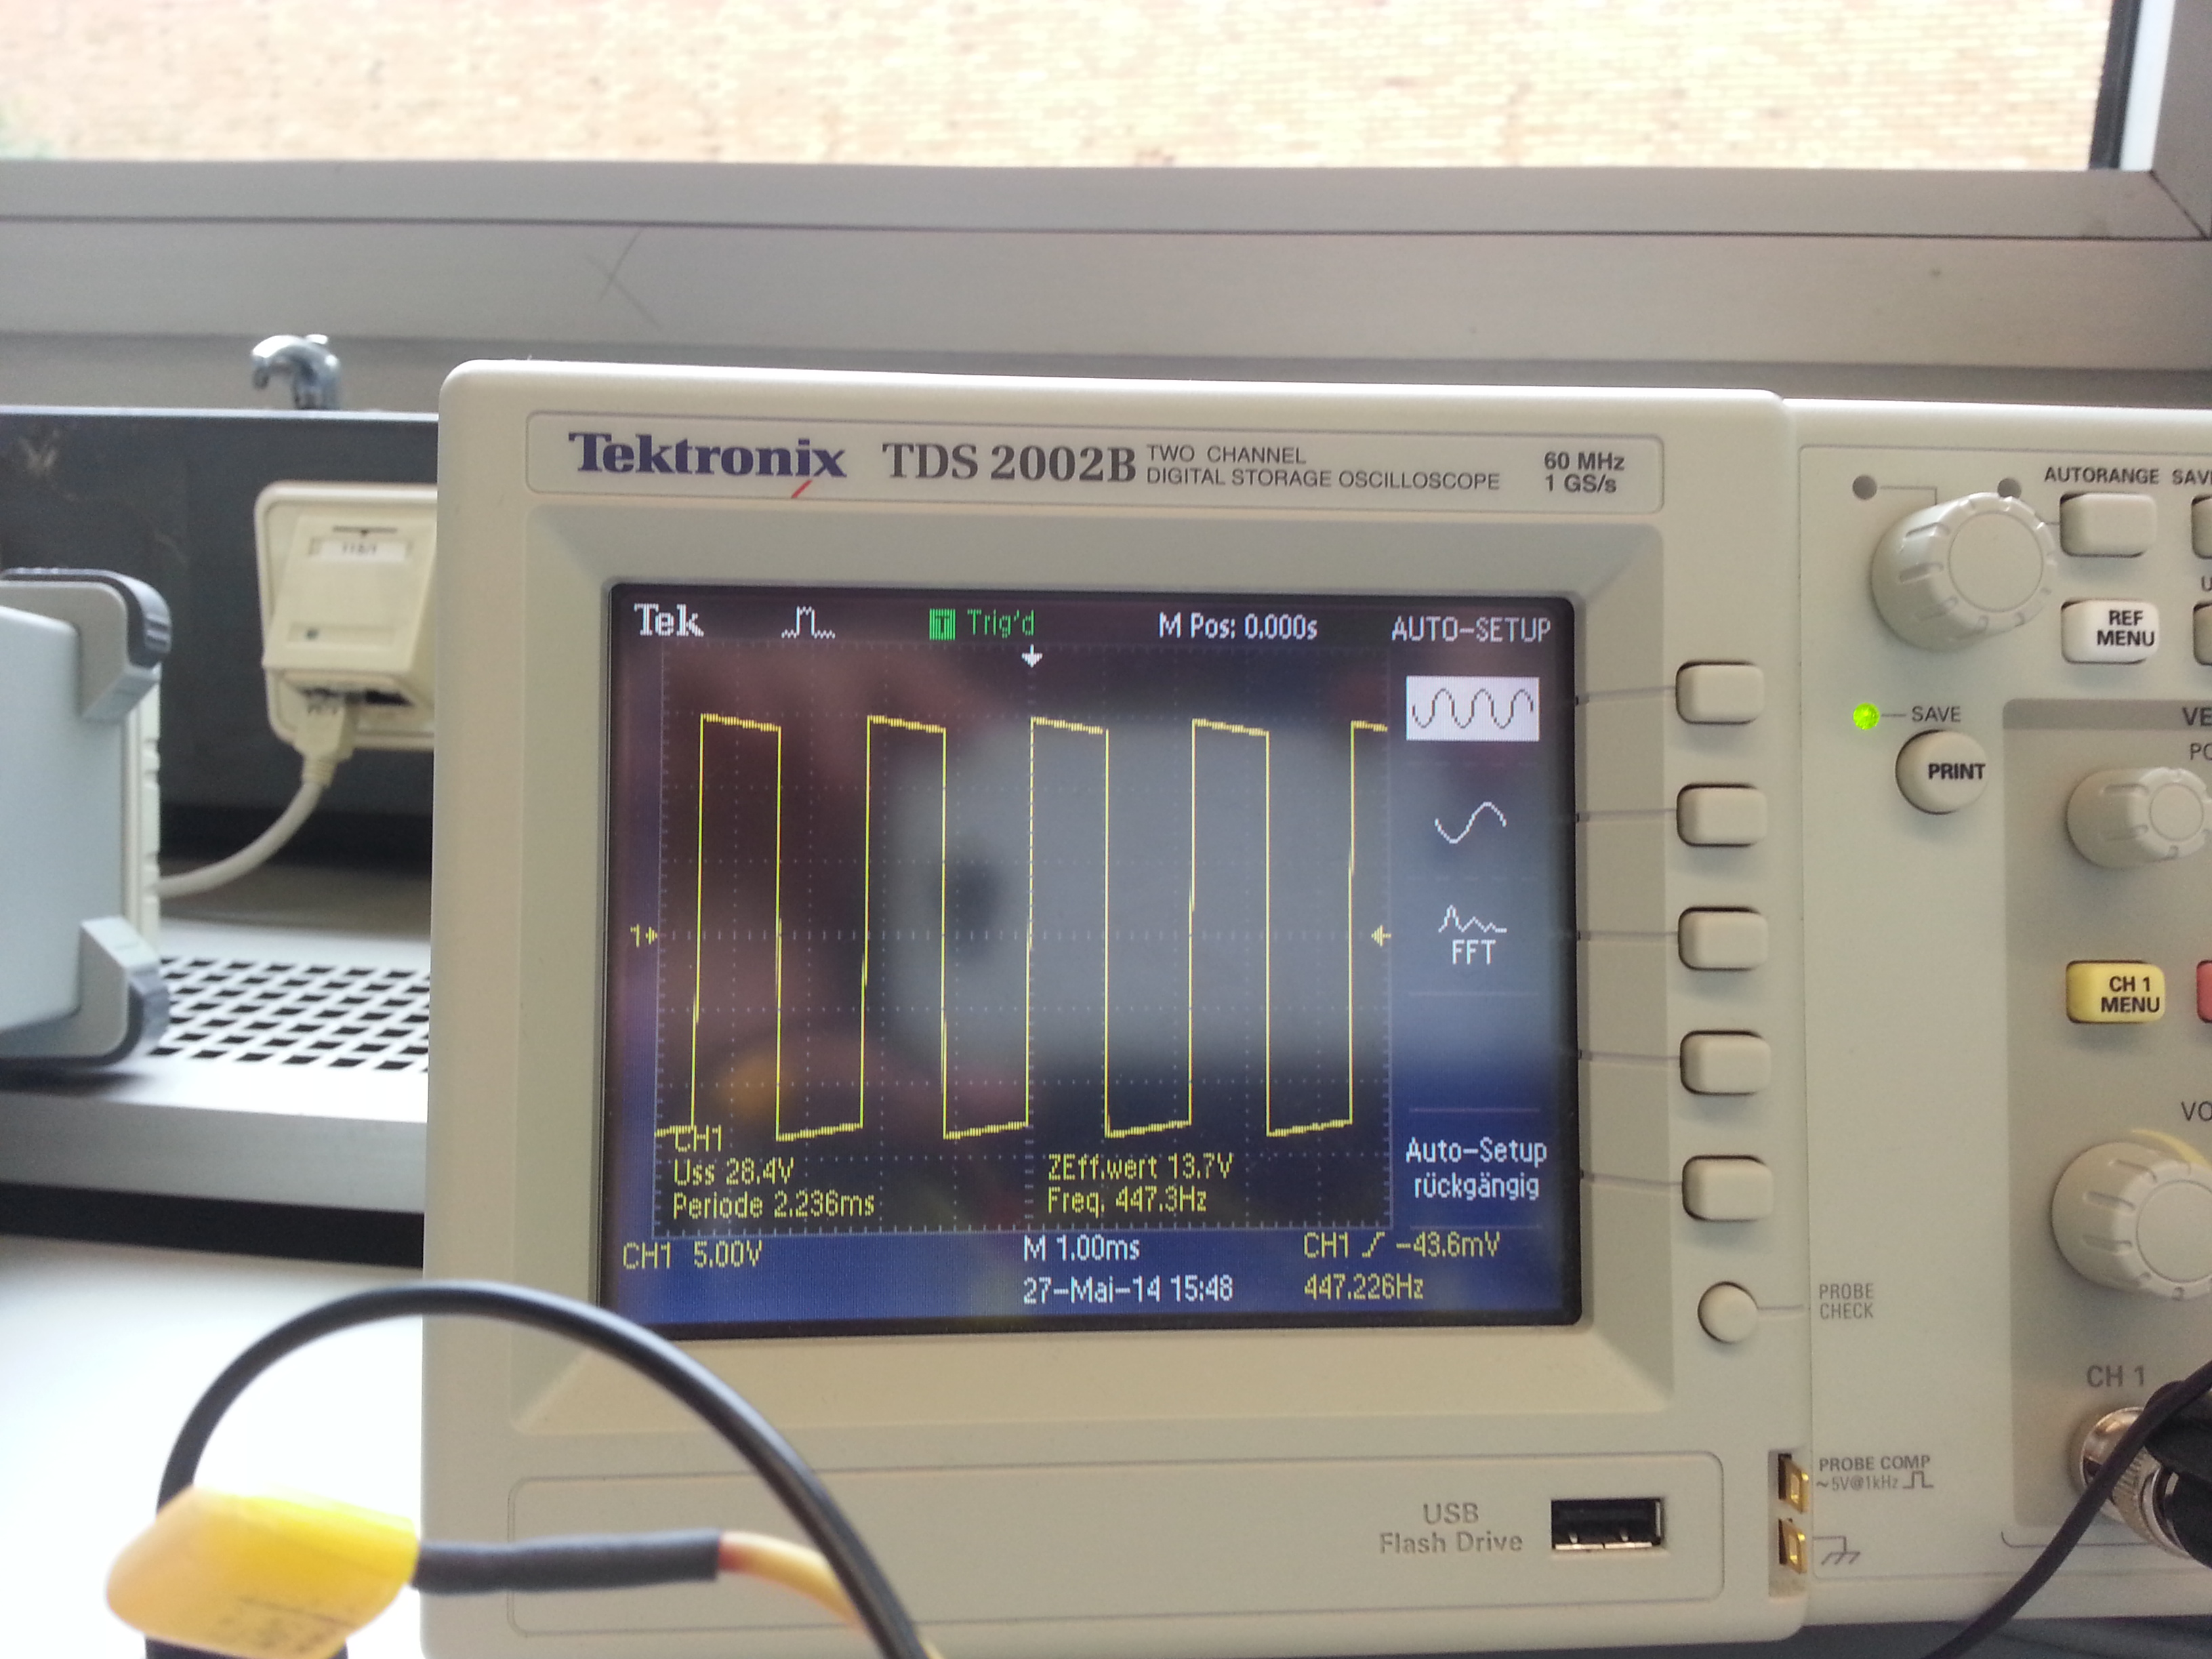
\includegraphics[scale=.08]{bilder/aufgabe_4_2_2.jpg} 
\caption{Generator: Rechteckssignal}
\end{figure}

\subsection{Programmierte Differentialgleichung 2.Ordnung}

Mit einer Schaltung aus OPV lässt sich auch eine Differentialgleichung 2. Ordnung simulieren. Hierbei handelt es sich um die Bewegungsgleichung einer harmonischen Schwingung. Durch variieren der Spannung (siehe Vorbereitung) konnten wir die verschiedenen Fälle der Lösung simulieren:

\begin{figure}[H]
\centering
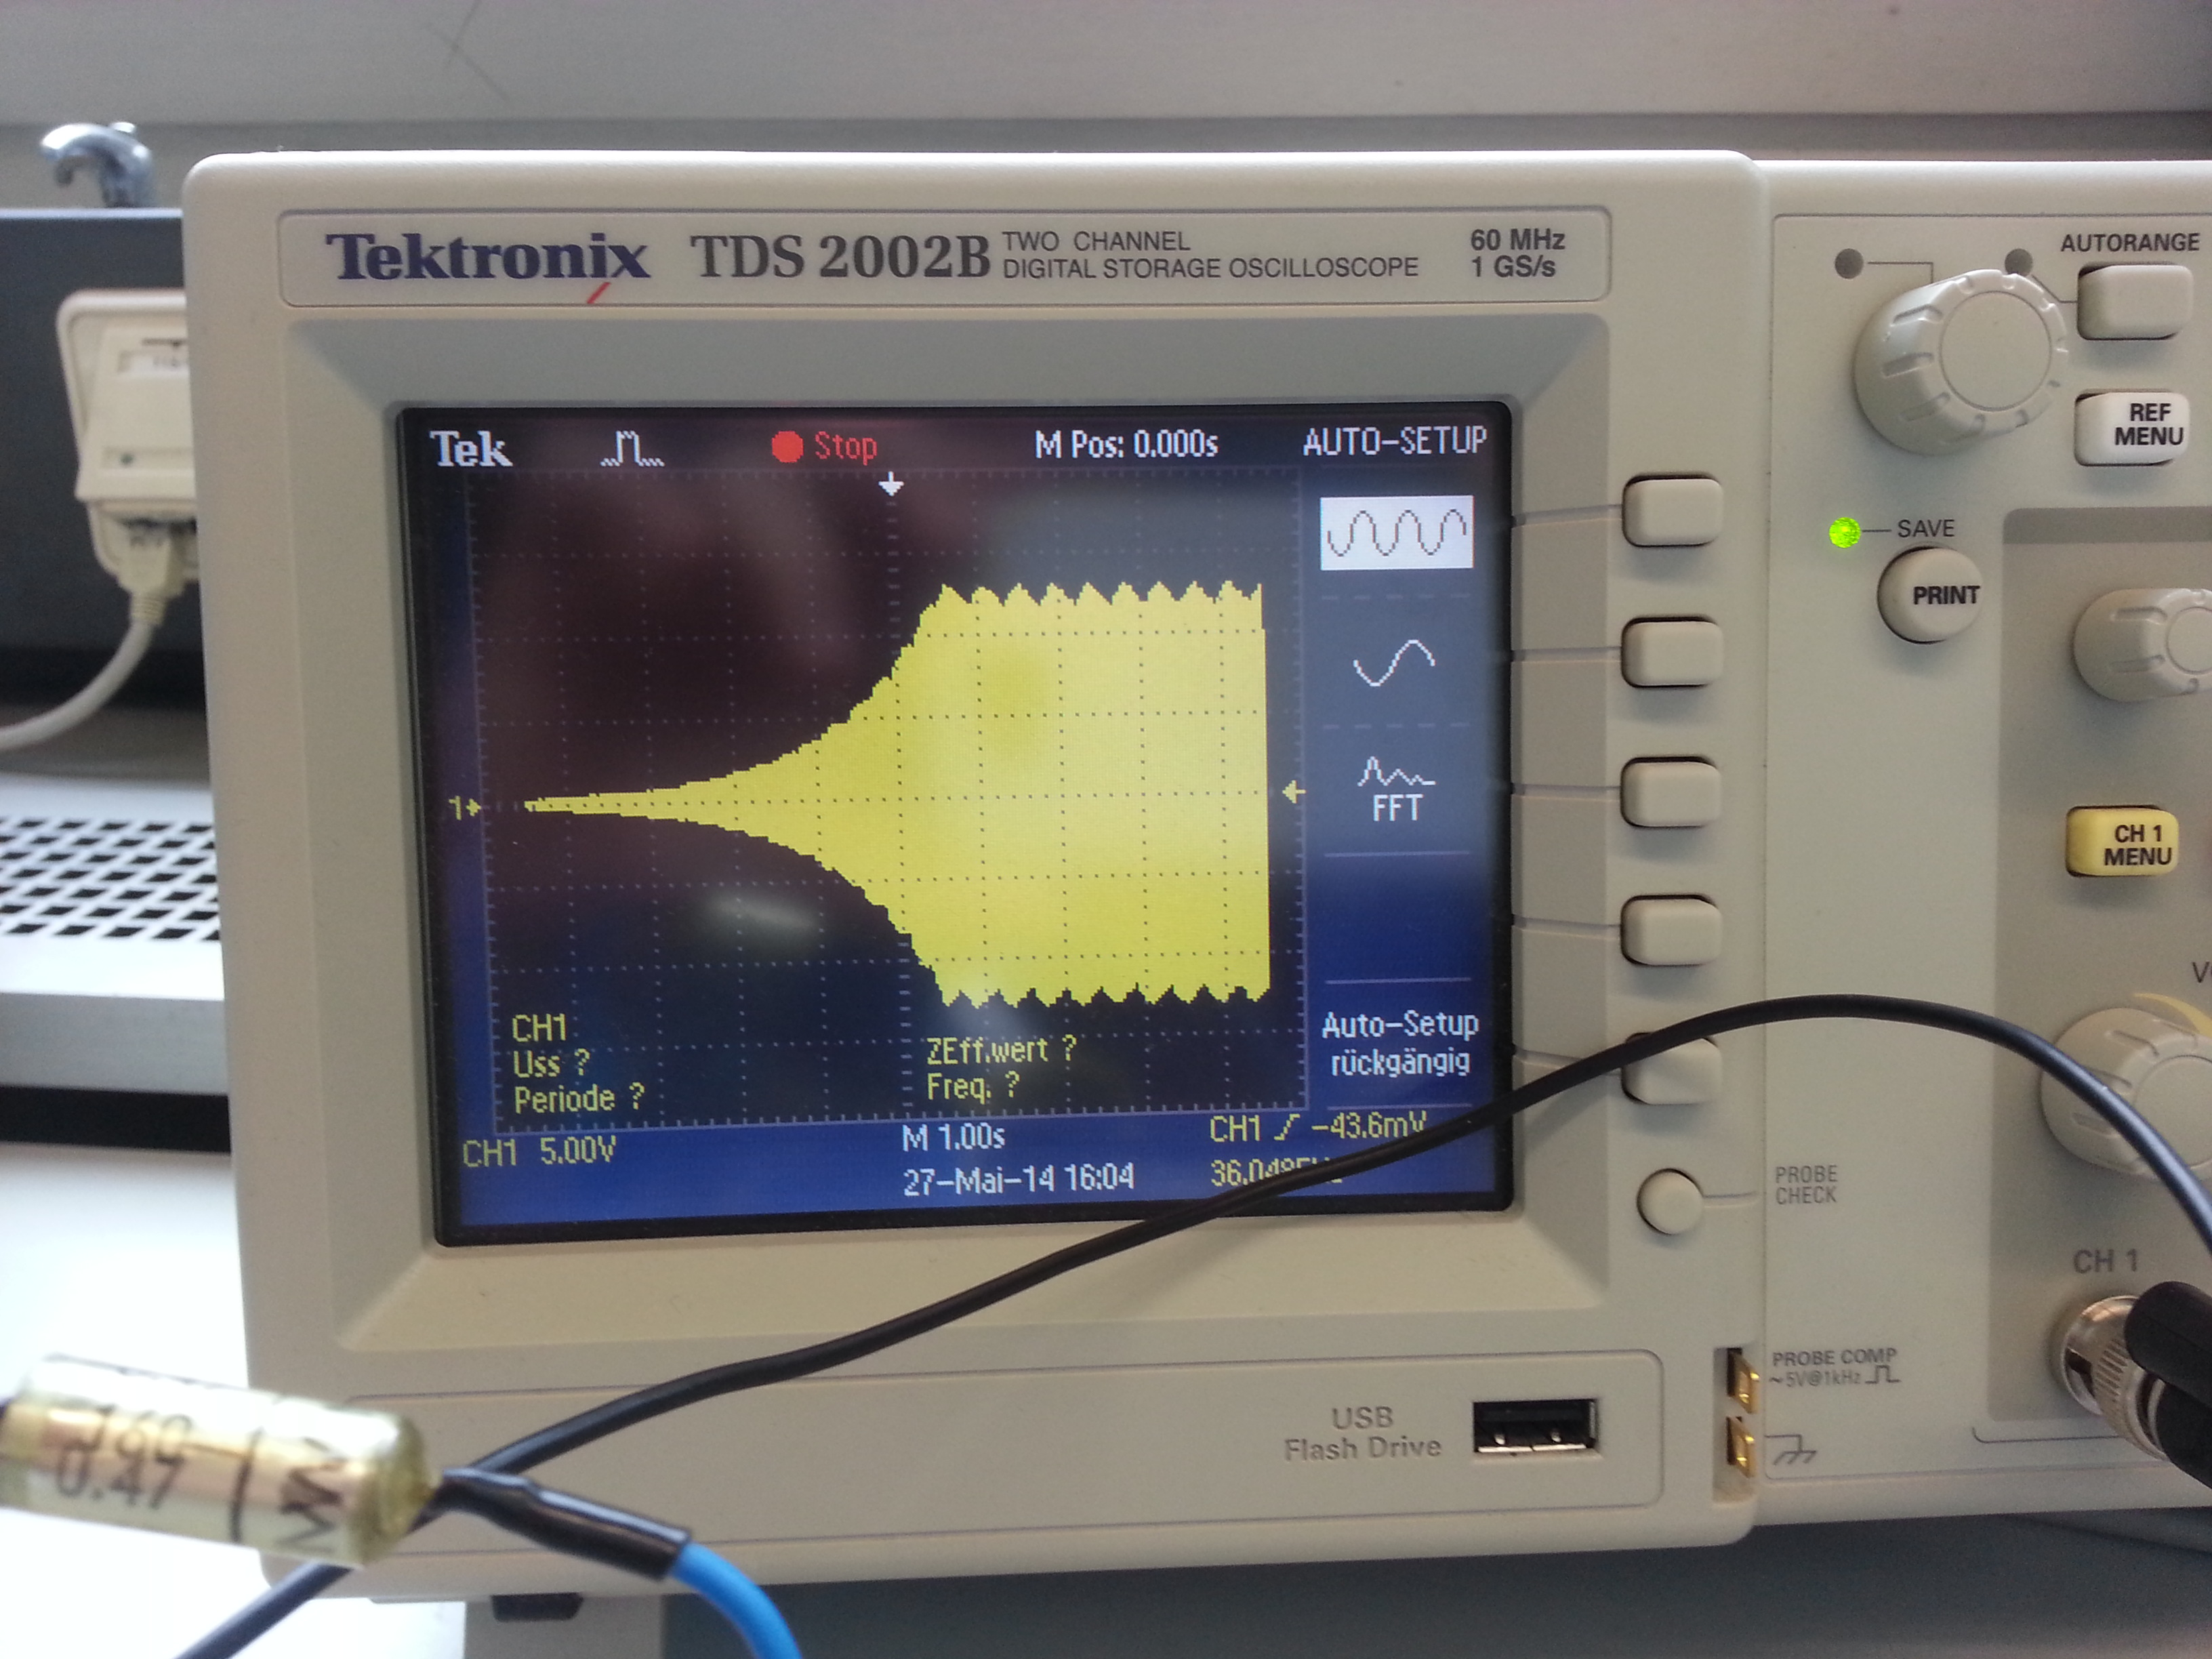
\includegraphics[scale=.08]{bilder/aufgabe_4_3_1.jpg} 
\caption{ungedämpfte Schwingung}
\end{figure}

\begin{figure}[H]
\centering
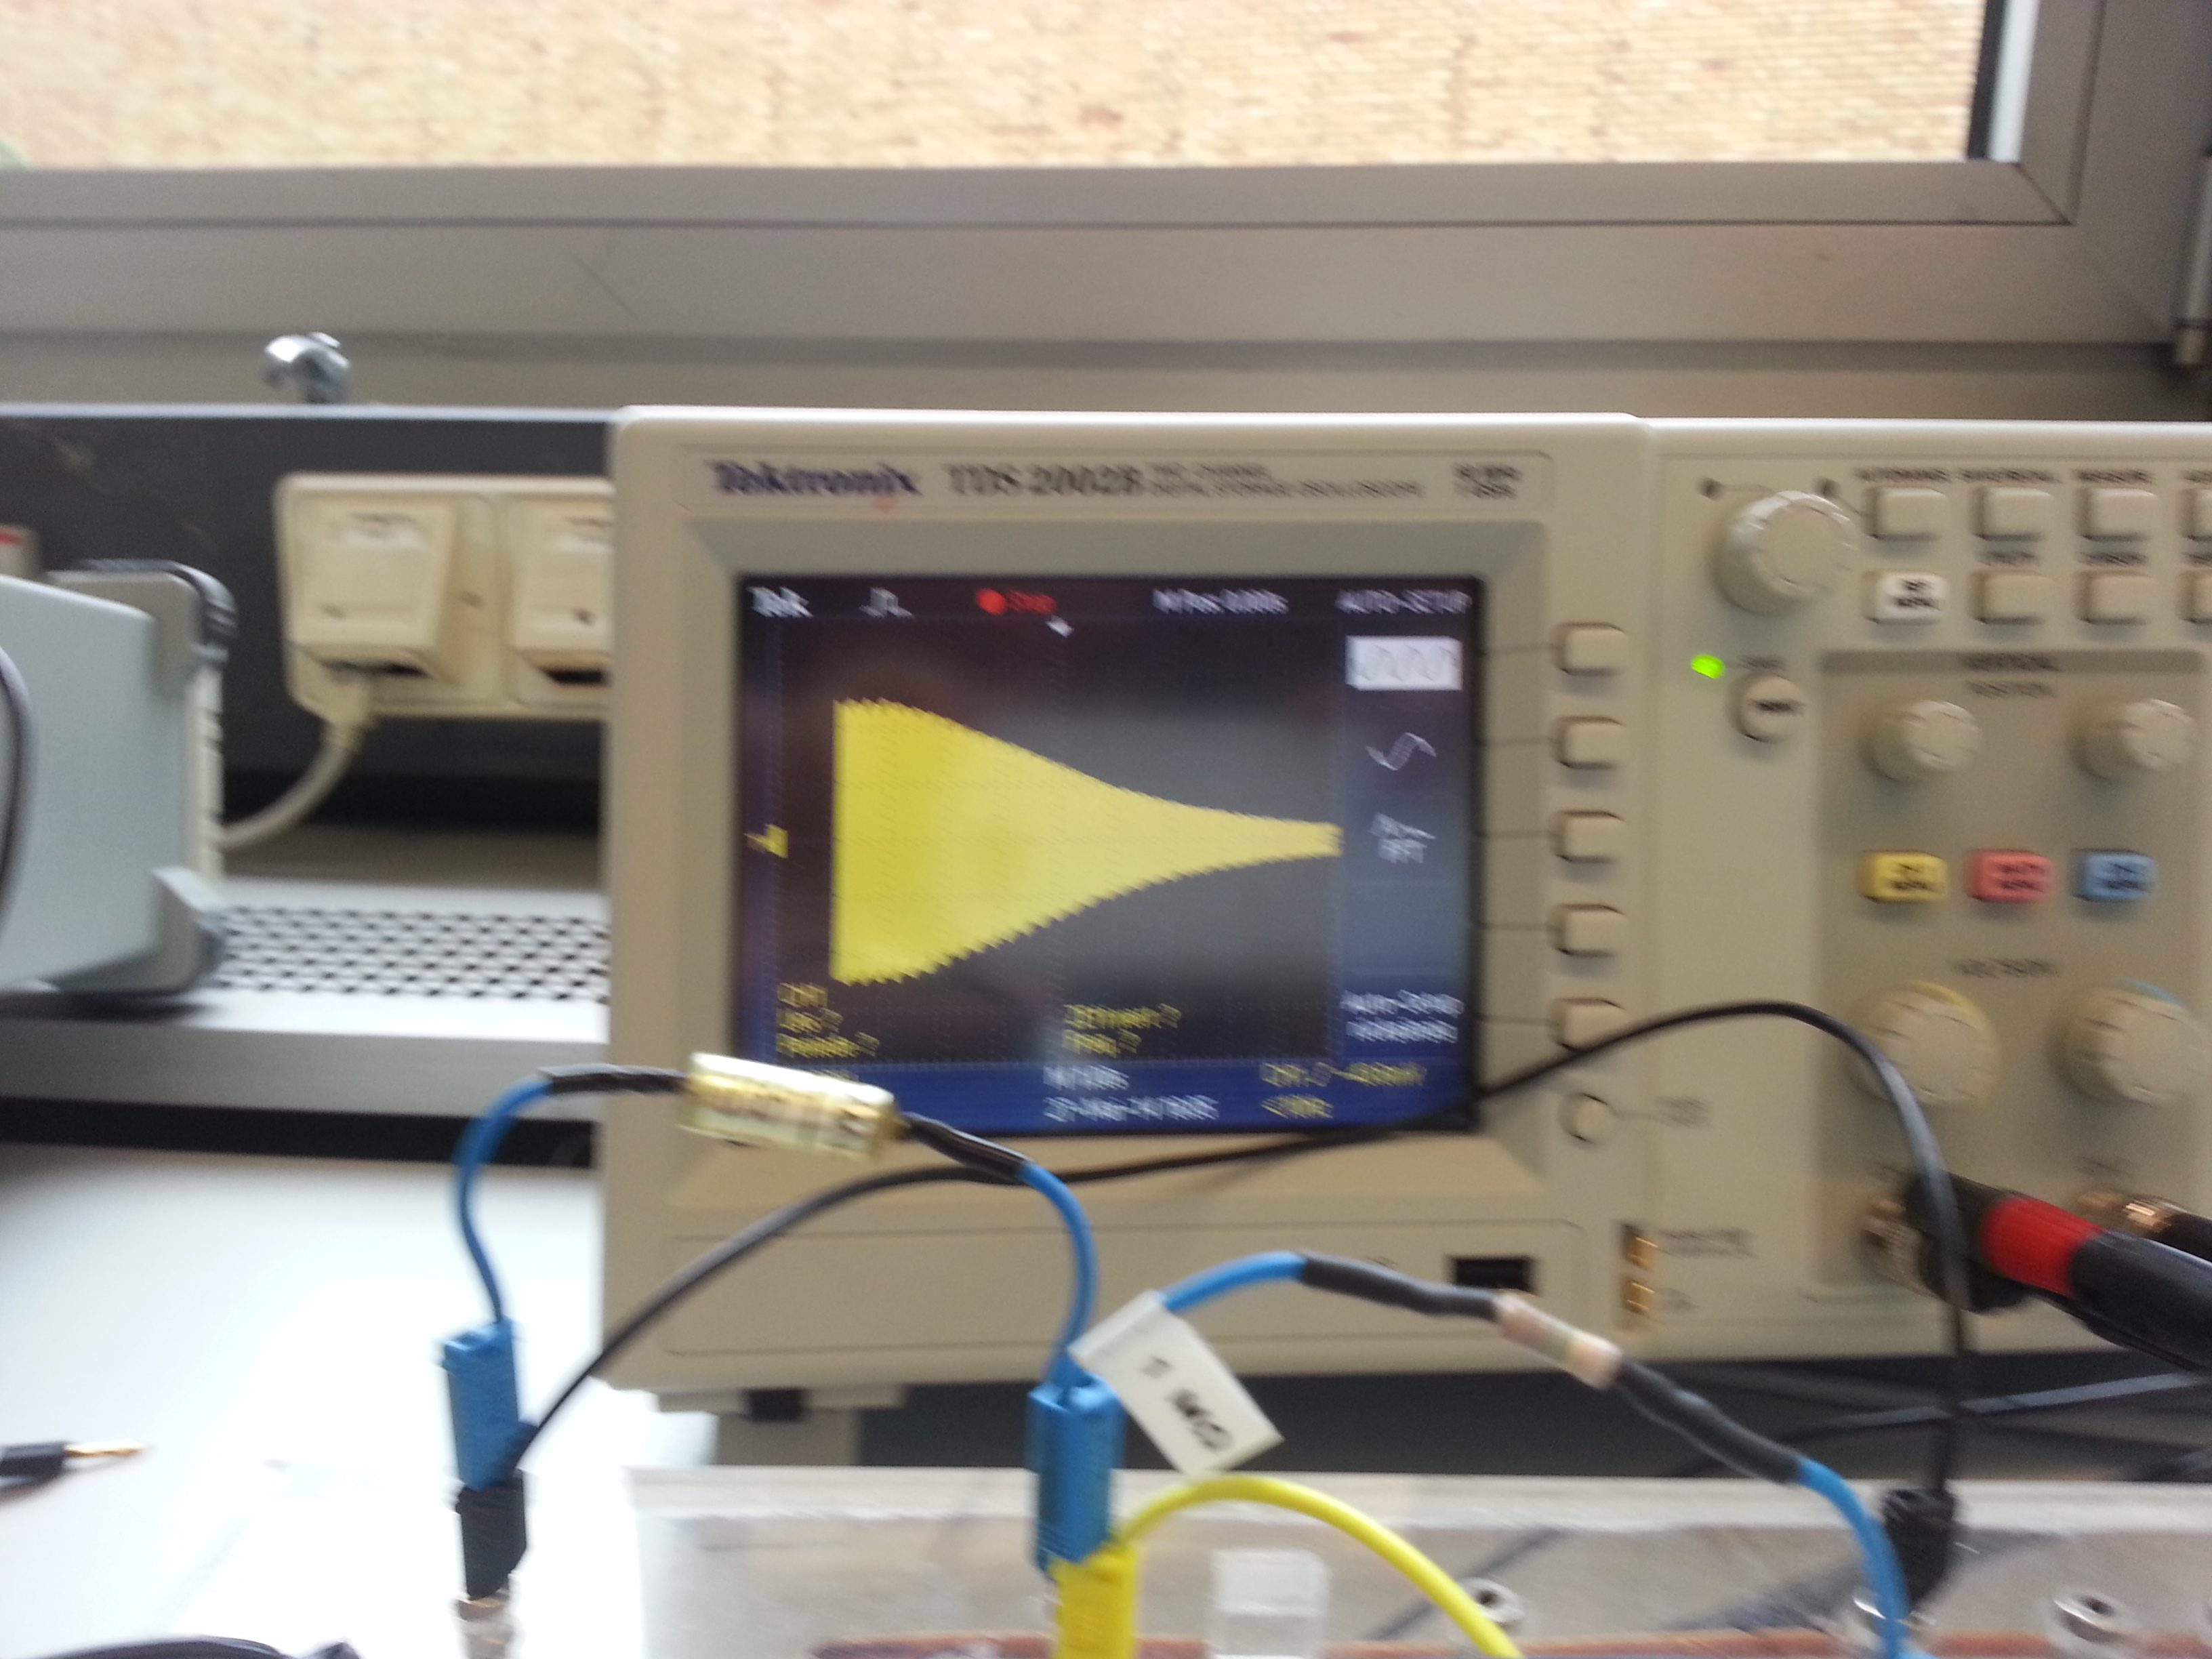
\includegraphics[scale=.08]{bilder/aufgabe_4_3_2.jpg} 
\caption{gedämpfte Schwingung}
\end{figure}

\begin{figure}[H]
\centering
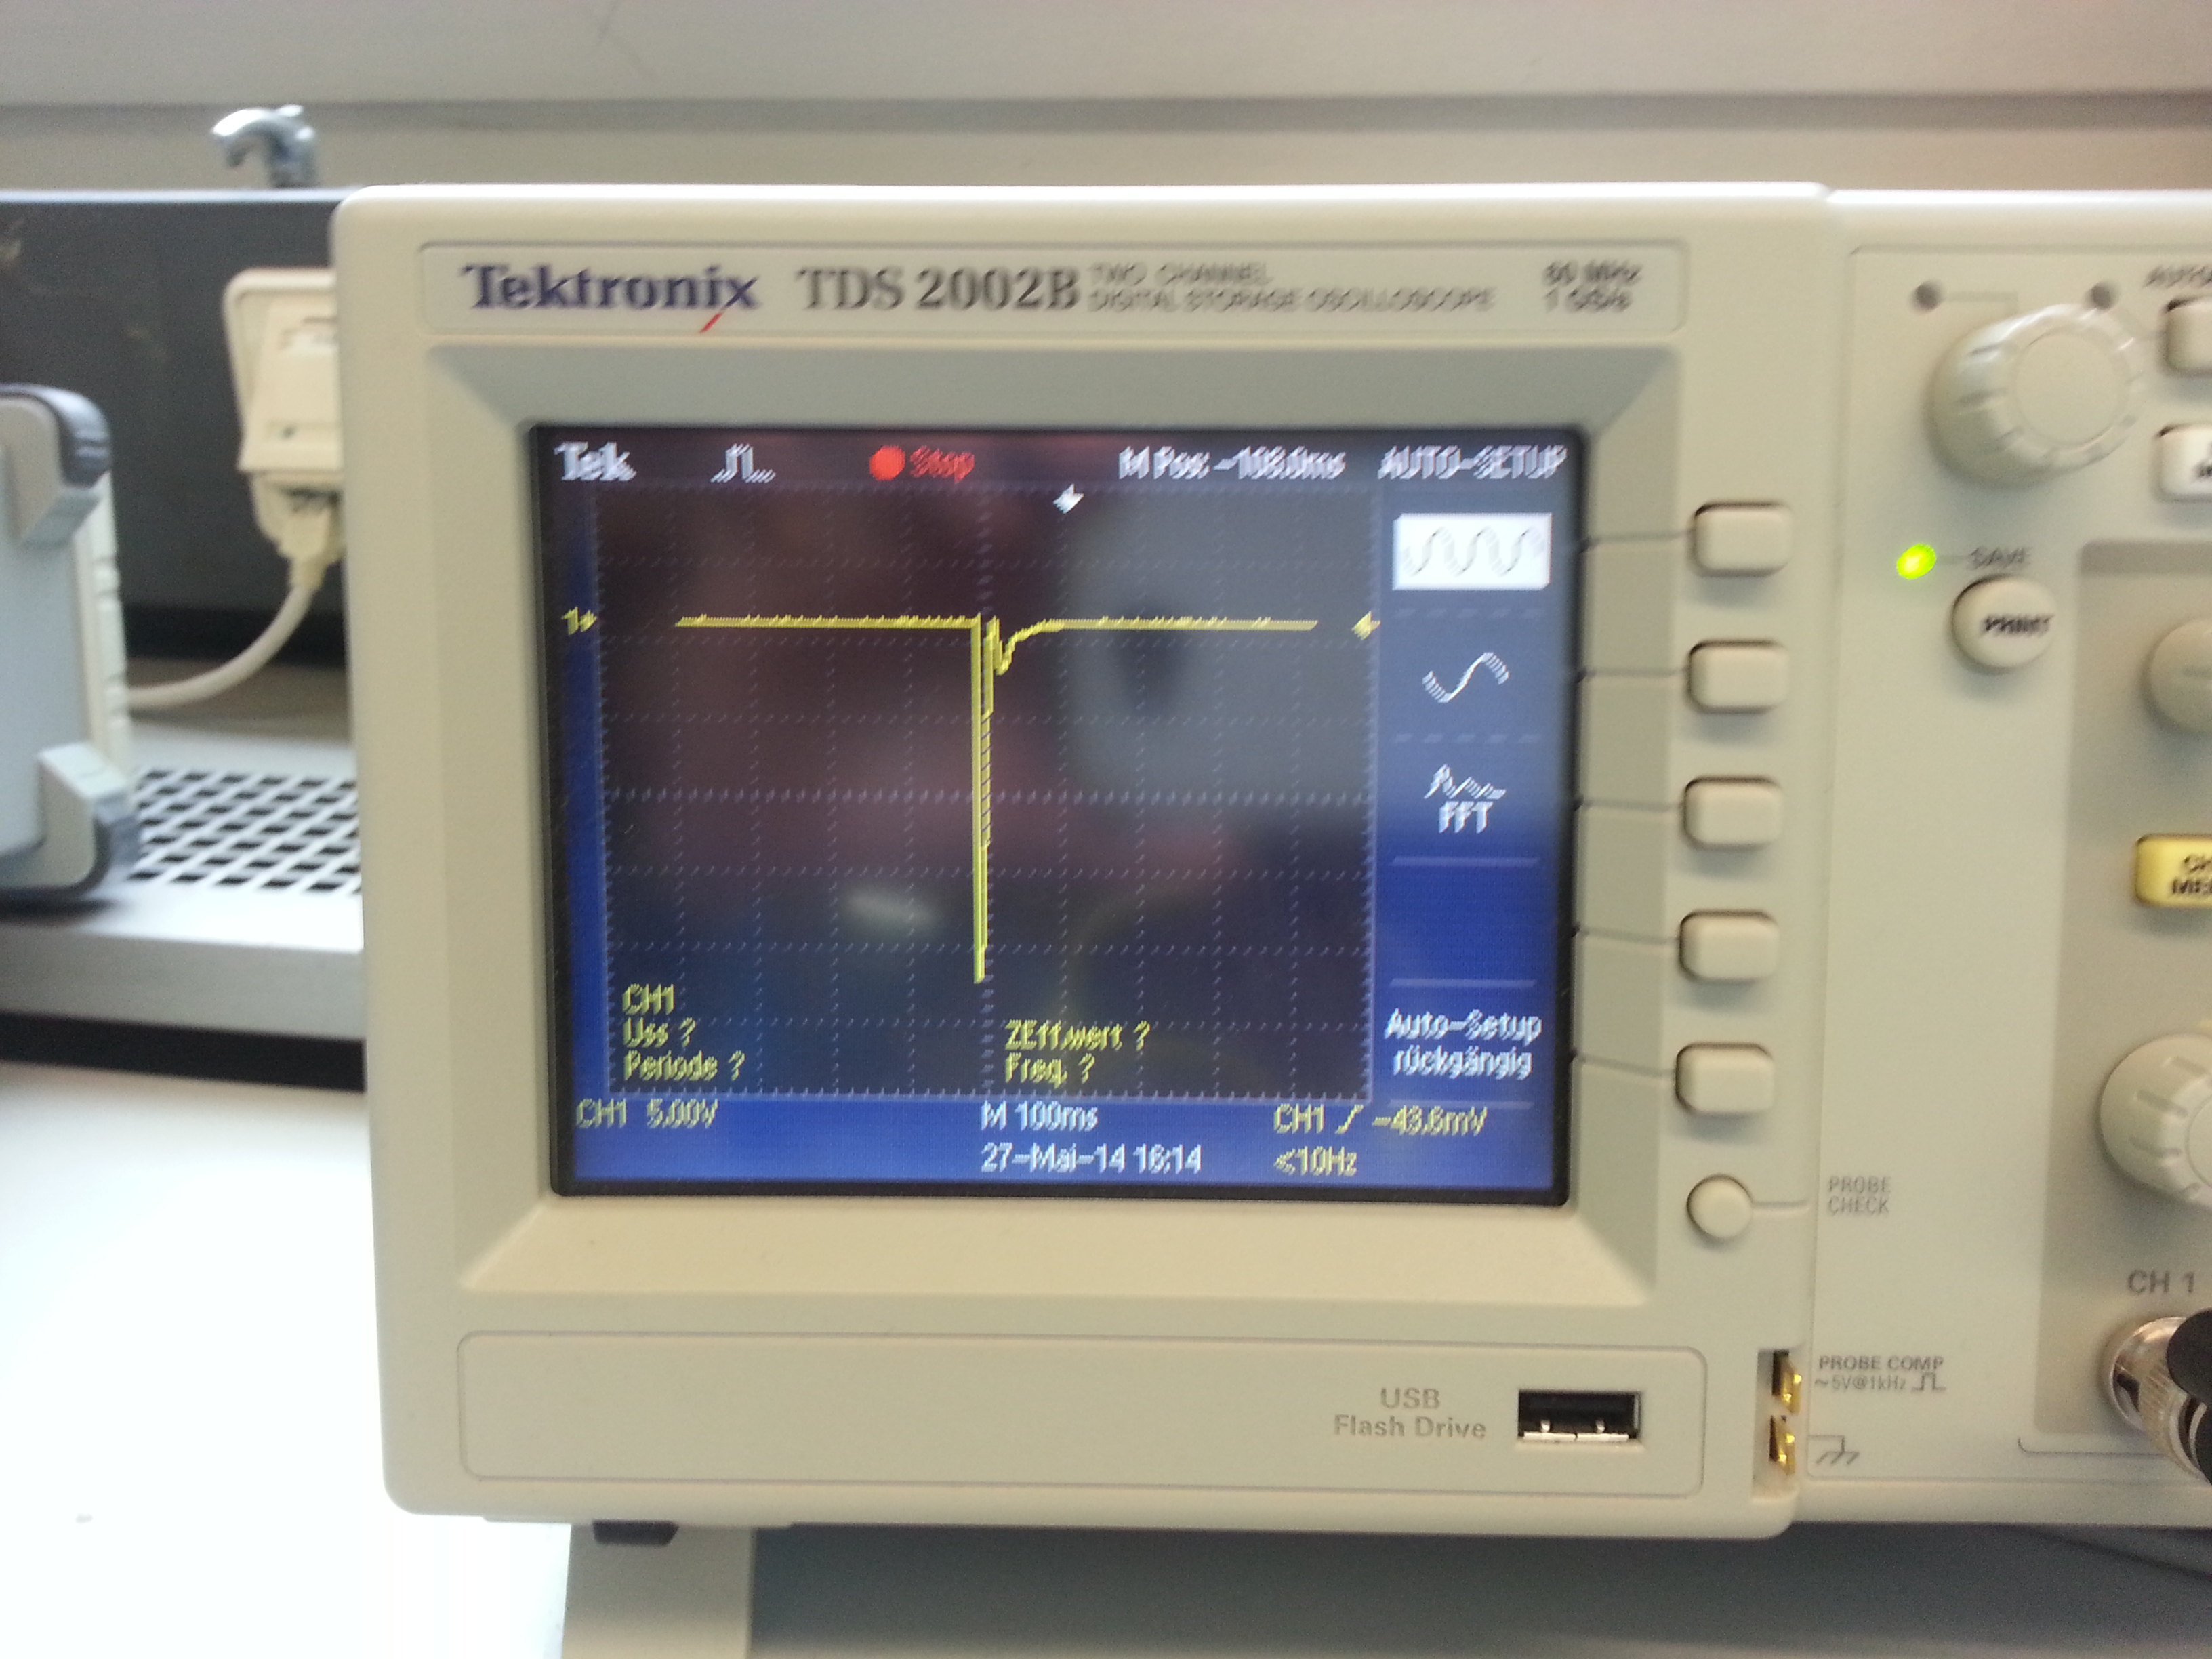
\includegraphics[scale=.08]{bilder/aufgabe_4_3_3.jpg} 
\caption{aperiodischer Grenzfall}
\end{figure}

Beim aperiodischen Grenzfall ist eigentlich eine Schwingung zu viel zusehen. Wir konnten die Spannung allerdings nicht präziser einstellen.
\end{document}